\documentclass[aps,pra,twocolumn,superscriptaddress,nofootinbib]{revtex4-2}
\usepackage{amsmath,amssymb,amsthm}
\usepackage{graphicx}
\usepackage{booktabs}
\usepackage{tikz}
\usetikzlibrary{positioning,arrows.meta,shapes.misc}
\usepackage[colorlinks=true,linkcolor=blue!50!black,citecolor=blue!50!black,urlcolor=blue!50!black]{hyperref}

\newtheorem{theorem}{Theorem}
\newtheorem{lemma}{Lemma}
% generated by sbpipe_study/make_figures.py -- do not edit
\newcommand{\dmrgEzeroErr}{2.3\times10^{-11}}
\newcommand{\dmrgEoneErr}{2.4\times10^{-11}}
\newcommand{\dmrgGammaErr}{4.0\times10^{-8}}
\newcommand{\weylErr}{1.2\times10^{-14}}
\newcommand{\nSim}{96}
\newcommand{\nSimOK}{96}
\newcommand{\nPlans}{144}
\newcommand{\boundRatioMin}{2.4}
\newcommand{\boundRatioMax}{4.0\times10^{5}}
\newcommand{\boundRatioMed}{14}
\newcommand{\leakRatioMin}{1.1}
\newcommand{\leakRatioMax}{1.3\times10^{5}}
\newcommand{\leakRatioMed}{4.3}
\newcommand{\trotRatioMin}{26}
\newcommand{\trotRatioMax}{4.5\times10^{3}}
\newcommand{\trotRatioMed}{185}
\newcommand{\psuccRatioMin}{1.00}
\newcommand{\psuccRatioMax}{1.00}
\newcommand{\nScaleFail}{14}
\newcommand{\nScale}{144}
\newcommand{\fitAOptTwoCnot}{6.1}
\newcommand{\fitAOptTwoSteps}{4.3}
\newcommand{\fitAOptOneCnot}{8.0}
\newcommand{\fitAOptOneSteps}{6.2}
\newcommand{\fitADyaTwoCnot}{4.9}
\newcommand{\fitADyaTwoSteps}{2.6}
\newcommand{\fitADyaOneCnot}{6.2}
\newcommand{\fitADyaOneSteps}{4.0}
\newcommand{\fitBOptTwoCnot}{6.3}
\newcommand{\fitBOptTwoSteps}{4.6}
\newcommand{\fitBOptOneCnot}{8.4}
\newcommand{\fitBOptOneSteps}{6.7}
\newcommand{\fitBDyaTwoCnot}{5.0}
\newcommand{\fitBDyaTwoSteps}{2.7}
\newcommand{\fitBDyaOneCnot}{6.5}
\newcommand{\fitBDyaOneSteps}{4.2}
\newcommand{\fitCOptTwoCnot}{4.9}
\newcommand{\fitCOptTwoSteps}{3.7}
\newcommand{\fitCOptOneCnot}{6.5}
\newcommand{\fitCOptOneSteps}{5.3}
\newcommand{\fitCDyaTwoCnot}{3.5}
\newcommand{\fitCDyaTwoSteps}{2.1}
\newcommand{\fitCDyaOneCnot}{4.6}
\newcommand{\fitCDyaOneSteps}{3.3}
\newcommand{\cnotFortyEight}{$2.7\times10^{8}$}
\newcommand{\tFortyEight}{$1.3\times10^{10}$}
\newcommand{\schedFortyEight}{dyadic}
\newcommand{\gainOrderMin}{17}
\newcommand{\gainOrderMax}{666}
\newcommand{\gainOrderMed}{93}
\newcommand{\gainOptMin}{0.7}
\newcommand{\gainOptMax}{3.7}
\newcommand{\gainOptMed}{2.9}
\newcommand{\nDyaWins}{1}
\newcommand{\nOptCmp}{29}
\newcommand{\qetuFail}{0}
\newcommand{\qetuN}{36}
\newcommand{\qetuDyaMed}{3.3}
\newcommand{\qetuDyaMin}{2.1}
\newcommand{\qetuDyaMax}{3.9}
\newcommand{\qetuOptMed}{1.00}
\newcommand{\qetuOptMin}{0.85}
\newcommand{\qetuOptMax}{4.3}
\newcommand{\qetuOptN}{29}
\newcommand{\qetuBestMed}{1.09}
\newcommand{\qetuFortyEight}{$8.2\times10^{7}$}
\newcommand{\qetuNSim}{24}
\newcommand{\qetuNSimOK}{24}
\newcommand{\qetuBoundMed}{7.5}
\newcommand{\qetuLeakMed}{1.3}
\newcommand{\drvGapExp}{1.50}
\newcommand{\drvGapExpMin}{1.44}
\newcommand{\drvGapExpMax}{1.60}
\newcommand{\drvGamExp}{1.13}
\newcommand{\drvGamExpMin}{1.03}
\newcommand{\drvGamExpMax}{1.19}
\newcommand{\drvGamRaw}{1.52}
\newcommand{\drvNExp}{1.7}
\newcommand{\drvNExpMin}{1.4}
\newcommand{\drvNExpMax}{1.8}
\newcommand{\drvValN}{120}
\newcommand{\drvValOk}{120}
\newcommand{\drvValMed}{0.06}
\newcommand{\drvValMax}{0.43}
\newcommand{\drvValNmax}{14}
\newcommand{\drvNPlans}{3328}
\newcommand{\drvGamSpread}{2\times10^{3}}
\newcommand{\empN}{675}
\newcommand{\empKone}{675}
\newcommand{\empDegRatio}{1.09}
\newcommand{\empDegRatioMax}{6.0}
\newcommand{\empCertRatio}{22}
\newcommand{\empCertRatioMin}{7}
\newcommand{\empCertRatioMax}{2\times10^{2}}
\newcommand{\empCertK}{16}
\newcommand{\empGamRaw}{1.21}
\newcommand{\empGamLog}{0.97}
\newcommand{\empGamCert}{1.45}
\newcommand{\empGapExp}{0.98}
\newcommand{\empGapDeg}{1.00}
\newcommand{\empGapCert}{1.38}
\newcommand{\empNMatch}{2.3}
\newcommand{\empNMatchCert}{2.1}
\newcommand{\empNMatchDeg}{1.1}
\newcommand{\empNFixed}{3.1}
\newcommand{\empNFixedCert}{3.2}
\newcommand{\empNFixedDeg}{1.9}
\newcommand{\empMatchJ}{0.384, 0.510, 0.539, 0.550, 0.555}
\newcommand{\regDirect}{53}
\newcommand{\regNone}{4}
\newcommand{\regTotal}{57}
\newcommand{\cylGamSixteen}{0.91}
\newcommand{\cylGamSixtyfour}{0.9994}
\newcommand{\actWins}{29}
\newcommand{\actRatioMax}{8.8}
\newcommand{\actRatioLo}{1.6}
\newcommand{\actOneWins}{18}
\newcommand{\actOneTot}{63}
\newcommand{\actOneLoss}{45}
\newcommand{\actOneRatioMax}{3.2}
\newcommand{\actOneFarMax}{8.8}
\newcommand{\actOneNearWins}{18}
\newcommand{\actOneNear}{31}
\newcommand{\actOneFar}{90}
\newcommand{\actOneNearPlusFar}{121}
\newcommand{\actOneFarMed}{20}
\newcommand{\goMDa}{10.1}
\newcommand{\goMDN}{1.50}
\newcommand{\goMDgap}{1.15}
\newcommand{\goMDL}{1.41}
\newcommand{\goMDrms}{1.23}
\newcommand{\goMDmax}{1.9}
\newcommand{\goMDgam}{0.78}
\newcommand{\goMOa}{9.81}
\newcommand{\goMON}{1.50}
\newcommand{\goMOgap}{1.36}
\newcommand{\goMOL}{1.24}
\newcommand{\goMOrms}{1.30}
\newcommand{\goMOmax}{2.3}
\newcommand{\goMOgam}{0.83}
\newcommand{\goMQa}{13.1}
\newcommand{\goMQN}{2.09}
\newcommand{\goMQgap}{0.74}
\newcommand{\goMQL}{0.68}
\newcommand{\goMQrms}{1.04}
\newcommand{\goMQmax}{1.2}
\newcommand{\goMQgam}{0.99}
\newcommand{\goCDa}{15}
\newcommand{\goCDN}{2.07}
\newcommand{\goCDgap}{1.27}
\newcommand{\goCDL}{2.43}
\newcommand{\goCDrms}{1.22}
\newcommand{\goCDmax}{2.2}
\newcommand{\goCDgam}{0.98}
\newcommand{\goCOa}{1.91}
\newcommand{\goCON}{2.27}
\newcommand{\goCOgap}{1.30}
\newcommand{\goCOL}{2.74}
\newcommand{\goCOrms}{1.45}
\newcommand{\goCOmax}{3.2}
\newcommand{\goCOgam}{0.97}
\newcommand{\goCQa}{9.53}
\newcommand{\goCQN}{2.03}
\newcommand{\goCQgap}{1.11}
\newcommand{\goCQL}{2.17}
\newcommand{\goCQrms}{1.22}
\newcommand{\goCQmax}{2.0}
\newcommand{\goCQgam}{0.99}
\newcommand{\goCertRatioMed}{62}
\newcommand{\goCertRatioMin}{14}
\newcommand{\goCertRatioMax}{258}
\newcommand{\goNcases}{222}
\newcommand{\goQetuOverDyMed}{1.26}
\newcommand{\fAMDcnot}{1.2--3.0}
\newcommand{\fBMDcnot}{2.7--4.3}
\newcommand{\fAMDtime}{1.5--3.0}
\newcommand{\fBMDtime}{1.5--2.8}
\newcommand{\fAMQcnot}{1.5--2.9}
\newcommand{\fBMQcnot}{1.7--1.9}
\newcommand{\fAMQtime}{1.5--2.9}
\newcommand{\fBMQtime}{1.8--2.1}
\newcommand{\fACDcnot}{4.6--9.4}
\newcommand{\fBCDcnot}{2.2--2.6}
\newcommand{\fACDtime}{1.5--3.0}
\newcommand{\fBCDtime}{1.7--2.3}
\newcommand{\fACQcnot}{4.2--7.1}
\newcommand{\fBCQcnot}{2.0--2.1}
\newcommand{\fACQtime}{1.5--2.5}
\newcommand{\fBCQtime}{1.8--2.0}
\newcommand{\fCMDtime}{2.0}
\newcommand{\fCMDtimeLo}{1.2}
\newcommand{\fCMDtimeHi}{3}
\newcommand{\fCMDsteps}{89.4}
\newcommand{\fCMDstepsLo}{26.2}
\newcommand{\fCMDstepsHi}{339}
\newcommand{\fCMQtime}{1.3}
\newcommand{\fCMQtimeLo}{1.0}
\newcommand{\fCMQtimeHi}{2}
\newcommand{\fCMQsteps}{19.2}
\newcommand{\fCMQstepsLo}{7.3}
\newcommand{\fCMQstepsHi}{68}
\newcommand{\fQDtime}{0.65}
\newcommand{\fQDsteps}{1.40}
\newcommand{\fRzCnot}{0.50}
\newcommand{\fCps}{20}
\newcommand{\fDtDTwo}{1.25}
\newcommand{\fDtCTwo}{0.017}
\newcommand{\fDtDThree}{0.56}
\newcommand{\fDtCThree}{0.009}
\newcommand{\fDtDFour}{0.30}
\newcommand{\fDtCFour}{0.005}
\newcommand{\fitMDTN}{-0.24}
\newcommand{\fitMDTgap}{1.19}
\newcommand{\fitMDTL}{0.77}
\newcommand{\fitMDTeps}{0.04}
\newcommand{\fitMDSN}{0.08}
\newcommand{\fitMDSgap}{1.90}
\newcommand{\fitMDSL}{0.71}
\newcommand{\fitMDSeps}{0.27}
\newcommand{\fitMDCN}{1.30}
\newcommand{\fitMDCgap}{1.89}
\newcommand{\fitMDCL}{0.71}
\newcommand{\fitMDCeps}{0.26}
\newcommand{\fitMQTN}{-0.10}
\newcommand{\fitMQTgap}{1.10}
\newcommand{\fitMQTL}{0.86}
\newcommand{\fitMQTeps}{0.01}
\newcommand{\fitMQSN}{1.02}
\newcommand{\fitMQSgap}{0.96}
\newcommand{\fitMQSL}{0.86}
\newcommand{\fitMQSeps}{0.01}
\newcommand{\fitMQCN}{2.22}
\newcommand{\fitMQCgap}{0.96}
\newcommand{\fitMQCL}{0.86}
\newcommand{\fitMQCeps}{0.01}
\newcommand{\fitCDTN}{0.04}
\newcommand{\fitCDTgap}{1.10}
\newcommand{\fitCDTL}{0.84}
\newcommand{\fitCDTeps}{0.01}
\newcommand{\fitCDSN}{0.85}
\newcommand{\fitCDSgap}{1.30}
\newcommand{\fitCDSL}{2.03}
\newcommand{\fitCDSeps}{0.12}
\newcommand{\fitCDCN}{2.08}
\newcommand{\fitCDCgap}{1.30}
\newcommand{\fitCDCL}{2.03}
\newcommand{\fitCDCeps}{0.12}
\newcommand{\fitCQTN}{0.01}
\newcommand{\fitCQTgap}{1.00}
\newcommand{\fitCQTL}{0.73}
\newcommand{\fitCQTeps}{0.01}
\newcommand{\fitCQSN}{0.81}
\newcommand{\fitCQSgap}{1.14}
\newcommand{\fitCQSL}{1.84}
\newcommand{\fitCQSeps}{0.12}
\newcommand{\fitCQCN}{2.04}
\newcommand{\fitCQCgap}{1.14}
\newcommand{\fitCQCL}{1.83}
\newcommand{\fitCQCeps}{0.12}
\newcommand{\optRetried}{21}
\newcommand{\optCertRetried}{10}
\newcommand{\optPoints}{286}
\newcommand{\odMMed}{0.89}
\newcommand{\odMLo}{0.58}
\newcommand{\odMHi}{1.55}
\newcommand{\odMWins}{169}
\newcommand{\odCMed}{0.35}
\newcommand{\odCLo}{0.27}
\newcommand{\odCHi}{1.05}
\newcommand{\odCWins}{221}
\newcommand{\optPgLo}{0.52}
\newcommand{\optPgMed}{0.88}
\newcommand{\bestDyTwo}{23}
\newcommand{\bestOpTwo}{51}
\newcommand{\bestQeTwo}{0}
\newcommand{\bestDyThree}{16}
\newcommand{\bestOpThree}{57}
\newcommand{\bestQeThree}{1}
\newcommand{\bestDyFour}{5}
\newcommand{\bestOpFour}{32}
\newcommand{\bestQeFour}{37}
\newcommand{\odShotTime}{0.58}
\newcommand{\odShotSteps}{0.62}
\newcommand{\odShotCnot}{0.63}
\newcommand{\fDtOFour}{0.30}
\newcommand{\fDtOTwo}{1.24}
\newcommand{\fitMOTN}{0.13}
\newcommand{\fitMOTgap}{1.21}
\newcommand{\fitMOTL}{1.19}
\newcommand{\fitMOTeps}{0.03}
\newcommand{\fitMOSN}{0.29}
\newcommand{\fitMOSgap}{1.84}
\newcommand{\fitMOSL}{1.05}
\newcommand{\fitMOSeps}{0.24}
\newcommand{\fitMOCN}{1.51}
\newcommand{\fitMOCgap}{1.83}
\newcommand{\fitMOCL}{1.05}
\newcommand{\fitMOCeps}{0.23}
\newcommand{\fitCOTN}{0.23}
\newcommand{\fitCOTgap}{1.24}
\newcommand{\fitCOTL}{1.02}
\newcommand{\fitCOTeps}{0.03}
\newcommand{\fitCOSN}{1.13}
\newcommand{\fitCOSgap}{1.46}
\newcommand{\fitCOSL}{2.39}
\newcommand{\fitCOSeps}{0.17}
\newcommand{\fitCOCN}{2.36}
\newcommand{\fitCOCgap}{1.46}
\newcommand{\fitCOCL}{2.39}
\newcommand{\fitCOCeps}{0.17}
\newcommand{\fCMOtime}{1.3}
\newcommand{\fCMOsteps}{39}
\newcommand{\goCertRatioOptMed}{26}
\newcommand{\goCertRatioOptMin}{5}
\newcommand{\goCertRatioOptMax}{185}
\newcommand{\goQetuWinsTwo}{0}
\newcommand{\goCasesTwo}{74}
\newcommand{\goQetuWinsThree}{9}
\newcommand{\goCasesThree}{74}
\newcommand{\goQetuWinsFour}{56}
\newcommand{\goCasesFour}{74}
\newcommand{\sensGapOneMiss}{0}
\newcommand{\sensGapOneTenMiss}{2}
\newcommand{\sensGapOneQuarterMiss}{10}
\newcommand{\sensGapOneHalfMiss}{16}
\newcommand{\sensGapN}{36}
\newcommand{\sensGapOneTenWorst}{$1.1\times10^{-2}$}
\newcommand{\sensDyaQuarterMiss}{0}
\newcommand{\sensGammaMiss}{12}
\newcommand{\sensGammaN}{72}
\newcommand{\sensGammaNoFilter}{12}
\newcommand{\gapFailFactor}{1.5}
\newcommand{\gapMarginCost}{2.9}
\newcommand{\gapMarginF}{0.5}
\newcommand{\gapWorstInf}{$5.1\times10^{-2}$}
\newcommand{\gapWorstF}{3}
\newcommand{\nGapFail}{3}
\newcommand{\eZeroHiCost}{13.5}
\newcommand{\eZeroHiF}{0.1}
\newcommand{\nEzeroFail}{0}
\newcommand{\nGammaFail}{0}
\newcommand{\gammaLowCost}{9.2}
\newcommand{\nAnsatzFail}{0}
\newcommand{\bestChiList}{4, 8}
\newcommand{\nNoFilter}{12}
\newcommand{\nNoFilterChiEight}{9}
\newcommand{\nChiEight}{9}
\newcommand{\cnotFortyEightChiFour}{$4.8\times10^{6}$}
\newcommand{\tFortyEightChiFour}{$2.1\times10^{8}$}
\newcommand{\cnotFortyEightChiEight}{4{,}500}
\newcommand{\gammaFortyEightChiEight}{0.9946}
\newcommand{\oracleMin}{8.7}
\newcommand{\oracleMax}{39}
\newcommand{\oracleMed}{21}
\newcommand{\cbestDyTwo}{0}
\newcommand{\cbestOpTwo}{38}
\newcommand{\cbestQeTwo}{36}
\newcommand{\cbestDyThree}{0}
\newcommand{\cbestOpThree}{25}
\newcommand{\cbestQeThree}{49}
\newcommand{\cbestDyFour}{0}
\newcommand{\cbestOpFour}{0}
\newcommand{\cbestQeFour}{74}
\newcommand{\cQetuBestTot}{159}
\newcommand{\cQetuOverDyMed}{0.30}
\newcommand{\cQetuWinsDy}{222}
\newcommand{\certOneWins}{0}
\newcommand{\certOneQWins}{0}
\newcommand{\certOneTot}{63}
\newcommand{\certOneOverMed}{152.3}
\newcommand{\certOneOverMin}{13.5}
\newcommand{\certOneRatioMax}{--}
\newcommand{\certTwoWins}{2}
\newcommand{\certTwoQWins}{3}
\newcommand{\certTwoTot}{28}
\newcommand{\certTwoOverMed}{5.2}
\newcommand{\certTwoOverMin}{1.0}
\newcommand{\certTwoRatioMax}{--}
\newcommand{\robQOneTwo}{27}
\newcommand{\robQOneOne}{18}
\newcommand{\robQHalfTwo}{25}
\newcommand{\robQHalfOne}{13}
\newcommand{\robQQuarterTwo}{23}
\newcommand{\robQQuarterOne}{6}
\newcommand{\robQEighthTwo}{19}
\newcommand{\robQEighthOne}{4}
\newcommand{\robQSixteenthTwo}{13}
\newcommand{\robQSixteenthOne}{0}
\newcommand{\robLbTwo}{16}
\newcommand{\robLbOne}{8}
\newcommand{\blQsdOne}{18}
\newcommand{\blQsdOneMax}{3.2}
\newcommand{\blQsdOneCert}{0}
\newcommand{\blQsdOneCertQ}{0}
\newcommand{\blQsdOneCertMed}{146.6}
\newcommand{\blQsdThree}{14}
\newcommand{\blQsdThreeMax}{7.8}
\newcommand{\blQsdThreeCert}{0}
\newcommand{\blQsdThreeCertQ}{1}
\newcommand{\blQsdThreeCertMed}{4.0}
\newcommand{\blQsdFour}{13}
\newcommand{\blQsdFourMax}{8.8}
\newcommand{\blQsdFourCert}{2}
\newcommand{\blQsdFourCertQ}{2}
\newcommand{\blQsdFourCertMed}{5.5}
\newcommand{\blAchOne}{16}
\newcommand{\blAchOneMax}{2.9}
\newcommand{\blAchOneCert}{0}
\newcommand{\blAchOneCertQ}{0}
\newcommand{\blAchOneCertMed}{176.9}
\newcommand{\blAchThree}{5}
\newcommand{\blAchThreeMax}{1.4}
\newcommand{\blAchThreeCert}{0}
\newcommand{\blAchThreeCertQ}{0}
\newcommand{\blAchThreeCertMed}{18.3}
\newcommand{\blAchFour}{13}
\newcommand{\blAchFourMax}{5.7}
\newcommand{\blAchFourCert}{0}
\newcommand{\blAchFourCertQ}{0}
\newcommand{\blAchFourCertMed}{8.5}
\newcommand{\blLbOne}{8}
\newcommand{\blLbOneMax}{2.1}
\newcommand{\blLbOneCert}{0}
\newcommand{\blLbOneCertQ}{0}
\newcommand{\blLbOneCertMed}{416.0}
\newcommand{\blLbThree}{3}
\newcommand{\blLbThreeMax}{1.7}
\newcommand{\blLbThreeCert}{0}
\newcommand{\blLbThreeCertQ}{0}
\newcommand{\blLbThreeCertMed}{33.4}
\newcommand{\blLbFour}{13}
\newcommand{\blLbFourMax}{3.2}
\newcommand{\blLbFourCert}{0}
\newcommand{\blLbFourCertQ}{0}
\newcommand{\blLbFourCertMed}{18.9}
\newcommand{\pbTwelve}{3\,831}
\newcommand{\glTwelve}{2\,039}
\newcommand{\pbFourteen}{15\,511}
\newcommand{\glFourteen}{8\,181}
\newcommand{\pbSixteen}{62\,423}
\newcommand{\glSixteen}{32\,756}
\newcommand{\tauPiMed}{0.68}
\newcommand{\tauPiMin}{0.29}
\newcommand{\tauPiMax}{4.28}
\newcommand{\tauTqMed}{0.75}
\newcommand{\tauNcases}{467}
\newcommand{\tauNgo}{222}
\newcommand{\tauBestDyTwo}{19}
\newcommand{\tauBestOpTwo}{48}
\newcommand{\tauBestQeTwo}{7}
\newcommand{\tauBestDyThree}{4}
\newcommand{\tauBestOpThree}{32}
\newcommand{\tauBestQeThree}{38}
\newcommand{\tauBestDyFour}{0}
\newcommand{\tauBestOpFour}{9}
\newcommand{\tauBestQeFour}{65}
\newcommand{\tauXOneWins}{14}
\newcommand{\tauXOneBest}{2}
\newcommand{\tauXTwoWins}{26}
\newcommand{\tauXTwoBest}{1}
\newcommand{\apN}{182}
\newcommand{\apEok}{182}
\newcommand{\apEtot}{182}
\newcommand{\apTok}{112}
\newcommand{\apTtot}{112}
\newcommand{\apOrCertS}{0.09}
\newcommand{\apEcertS}{0.22}
\newcommand{\apEorS}{1.9}
\newcommand{\apTcertS}{0.13}
\newcommand{\apTorS}{1.7}
\newcommand{\apOrCertQ}{0.12}
\newcommand{\apEcertQ}{0.23}
\newcommand{\apEorQ}{1.9}
\newcommand{\apTcertQ}{0.18}
\newcommand{\apTorQ}{1.9}
\newcommand{\apShotsMin}{4\times10^{5}}
\newcommand{\apShotsMax}{5\times10^{14}}
\newcommand{\apShotsMed}{2\times10^{10}}
\newcommand{\apCkMed}{6\times10^{9}}
\newcommand{\apXQOneE}{0}
\newcommand{\apXQOneT}{0}
\newcommand{\apXQOneTot}{63}
\newcommand{\apXQOneTtot}{42}
\newcommand{\apXQOneMax}{--}
\newcommand{\apXQOneTMax}{--}
\newcommand{\apXQThreeE}{5}
\newcommand{\apXQThreeT}{0}
\newcommand{\apXQThreeTot}{14}
\newcommand{\apXQThreeTtot}{0}
\newcommand{\apXQThreeMax}{2.2}
\newcommand{\apXQThreeTMax}{--}
\newcommand{\apXQFourE}{7}
\newcommand{\apXQFourT}{12}
\newcommand{\apXQFourTot}{14}
\newcommand{\apXQFourTtot}{14}
\newcommand{\apXQFourMax}{2.0}
\newcommand{\apXQFourTMax}{2.6}
\newcommand{\apXAOneE}{0}
\newcommand{\apXAOneT}{0}
\newcommand{\apXAOneTot}{63}
\newcommand{\apXAOneTtot}{42}
\newcommand{\apXAOneMax}{--}
\newcommand{\apXAOneTMax}{--}
\newcommand{\apXAThreeE}{0}
\newcommand{\apXAThreeT}{0}
\newcommand{\apXAThreeTot}{14}
\newcommand{\apXAThreeTtot}{0}
\newcommand{\apXAThreeMax}{--}
\newcommand{\apXAThreeTMax}{--}
\newcommand{\apXAFourE}{3}
\newcommand{\apXAFourT}{5}
\newcommand{\apXAFourTot}{14}
\newcommand{\apXAFourTtot}{14}
\newcommand{\apXAFourMax}{1.3}
\newcommand{\apXAFourTMax}{1.8}
\newcommand{\extTrQlo}{15}
\newcommand{\extTrAlo}{13}
\newcommand{\extTrStraddle}{5}
\newcommand{\extTrQ}{17}
\newcommand{\extTrA}{15}
\newcommand{\extTrTot}{18}
\newcommand{\extTrOnly}{4}
\newcommand{\cmQOneGrid}{18}
\newcommand{\cmQOneGridT}{0}
\newcommand{\cmOneTot}{63}
\newcommand{\cmOneTtot}{42}
\newcommand{\cmQThreeGrid}{14}
\newcommand{\cmQThreeGridT}{0}
\newcommand{\cmThreeTot}{14}
\newcommand{\cmThreeTtot}{0}
\newcommand{\cmQFourGrid}{13}
\newcommand{\cmQFourGridT}{12}
\newcommand{\cmFourTot}{14}
\newcommand{\cmFourTtot}{14}
\newcommand{\cmQOneAll}{18}
\newcommand{\cmQOneAllT}{0}
\newcommand{\cmQThreeAll}{14}
\newcommand{\cmQThreeAllT}{0}
\newcommand{\cmQFourAll}{13}
\newcommand{\cmQFourAllT}{12}
\newcommand{\cmAOneGrid}{16}
\newcommand{\cmAOneGridT}{0}
\newcommand{\cmAThreeGrid}{5}
\newcommand{\cmAThreeGridT}{0}
\newcommand{\cmAFourGrid}{13}
\newcommand{\cmAFourGridT}{5}
\newcommand{\cmAOneAll}{16}
\newcommand{\cmAOneAllT}{0}
\newcommand{\cmAThreeAll}{5}
\newcommand{\cmAThreeAllT}{0}
\newcommand{\cmAFourAll}{13}
\newcommand{\cmAFourAllT}{5}
\newcommand{\cmLOneGrid}{8}
\newcommand{\cmLOneGridT}{0}
\newcommand{\cmLThreeGrid}{3}
\newcommand{\cmLThreeGridT}{0}
\newcommand{\cmLFourGrid}{13}
\newcommand{\cmLFourGridT}{1}
\newcommand{\cmLOneAll}{0}
\newcommand{\cmLOneAllT}{0}
\newcommand{\cmLThreeAll}{2}
\newcommand{\cmLThreeAllT}{0}
\newcommand{\cmLFourAll}{13}
\newcommand{\cmLFourAllT}{0}
\newcommand{\jtOk}{308}
\newcommand{\jtTot}{308}
\newcommand{\jtChanged}{90}
\newcommand{\jtBeyond}{0}
\newcommand{\szShrink}{14}
\newcommand{\szTot}{112}
\newcommand{\twOk}{30}
\newcommand{\twTot}{30}
\newcommand{\twPrev}{28}
\newcommand{\twCert}{0.12}

\newcommand{\bdCommHi}{152}
\newcommand{\bdCommLo}{8}
\newcommand{\bdCommMed}{51}
\newcommand{\bdCommOptimizedMed}{39}
\newcommand{\bdCommQetuMed}{14}
\newcommand{\bdMKHi}{844897}
\newcommand{\bdMKLo}{42618}
\newcommand{\bdMKMed}{242855}
\newcommand{\bdMKvalid}{0.0034}
\newcommand{\bdMKvalidHi}{0.0042}
\newcommand{\blChainGen}{0}
\newcommand{\blChainGenHalf}{0}
\newcommand{\blChainTot}{63}
\newcommand{\blChainWins}{18}
\newcommand{\blChainWinsHalf}{13}
\newcommand{\blCylGen}{11}
\newcommand{\blCylGenHalf}{7}
\newcommand{\blCylTot}{28}
\newcommand{\blCylWins}{27}
\newcommand{\blCylWinsHalf}{25}
\newcommand{\ciDShotN}{1.31}
\newcommand{\ciDShotNhi}{1.49}
\newcommand{\ciDShotNlo}{1.12}
\newcommand{\ciDShota}{0.562}
\newcommand{\ciDShoteps}{2.40}
\newcommand{\ciDShotepshi}{2.57}
\newcommand{\ciDShotepslo}{2.22}
\newcommand{\ciDShotgam}{0.14}
\newcommand{\ciDShotgamhi}{0.16}
\newcommand{\ciDShotgamlo}{0.12}
\newcommand{\ciDShotgap}{1.91}
\newcommand{\ciDShotgaphi}{2.16}
\newcommand{\ciDShotgaplo}{1.60}
\newcommand{\ciDShotrms}{1.24}
\newcommand{\ciDSuccN}{1.42}
\newcommand{\ciDSuccNhi}{1.61}
\newcommand{\ciDSuccNlo}{1.23}
\newcommand{\ciDSucca}{0.639}
\newcommand{\ciDSucceps}{2.29}
\newcommand{\ciDSuccepshi}{2.47}
\newcommand{\ciDSuccepslo}{2.10}
\newcommand{\ciDSuccgam}{1.14}
\newcommand{\ciDSuccgamhi}{1.16}
\newcommand{\ciDSuccgamlo}{1.11}
\newcommand{\ciDSuccgap}{1.72}
\newcommand{\ciDSuccgaphi}{1.96}
\newcommand{\ciDSuccgaplo}{1.43}
\newcommand{\ciDSuccrms}{1.25}
\newcommand{\ciDTotN}{1.52}
\newcommand{\ciDTotNhi}{1.66}
\newcommand{\ciDTotNlo}{1.37}
\newcommand{\ciDTota}{5.34}
\newcommand{\ciDToteps}{1.54}
\newcommand{\ciDTotepshi}{1.70}
\newcommand{\ciDTotepslo}{1.36}
\newcommand{\ciDTotgam}{1.08}
\newcommand{\ciDTotgamhi}{1.10}
\newcommand{\ciDTotgamlo}{1.07}
\newcommand{\ciDTotgap}{1.19}
\newcommand{\ciDTotgaphi}{1.37}
\newcommand{\ciDTotgaplo}{0.99}
\newcommand{\ciDTotrms}{1.19}
\newcommand{\ciNcases}{222}
\newcommand{\ciNsys}{21}
\newcommand{\ciOShotN}{1.52}
\newcommand{\ciOShotNhi}{1.71}
\newcommand{\ciOShotNlo}{1.30}
\newcommand{\ciOShota}{0.156}
\newcommand{\ciOShoteps}{2.52}
\newcommand{\ciOShotepshi}{2.68}
\newcommand{\ciOShotepslo}{2.37}
\newcommand{\ciOShotgam}{0.27}
\newcommand{\ciOShotgamhi}{0.28}
\newcommand{\ciOShotgamlo}{0.25}
\newcommand{\ciOShotgap}{1.86}
\newcommand{\ciOShotgaphi}{2.07}
\newcommand{\ciOShotgaplo}{1.58}
\newcommand{\ciOShotrms}{1.26}
\newcommand{\ciOSuccN}{1.45}
\newcommand{\ciOSuccNhi}{1.63}
\newcommand{\ciOSuccNlo}{1.27}
\newcommand{\ciOSucca}{0.248}
\newcommand{\ciOSucceps}{2.44}
\newcommand{\ciOSuccepshi}{2.60}
\newcommand{\ciOSuccepslo}{2.29}
\newcommand{\ciOSuccgam}{1.20}
\newcommand{\ciOSuccgamhi}{1.21}
\newcommand{\ciOSuccgamlo}{1.18}
\newcommand{\ciOSuccgap}{2.01}
\newcommand{\ciOSuccgaphi}{2.19}
\newcommand{\ciOSuccgaplo}{1.76}
\newcommand{\ciOSuccrms}{1.23}
\newcommand{\ciOTotN}{1.52}
\newcommand{\ciOTotNhi}{1.64}
\newcommand{\ciOTotNlo}{1.41}
\newcommand{\ciOTota}{4.57}
\newcommand{\ciOToteps}{1.46}
\newcommand{\ciOTotepshi}{1.62}
\newcommand{\ciOTotepslo}{1.32}
\newcommand{\ciOTotgam}{1.09}
\newcommand{\ciOTotgamhi}{1.10}
\newcommand{\ciOTotgamlo}{1.09}
\newcommand{\ciOTotgap}{1.39}
\newcommand{\ciOTotgaphi}{1.52}
\newcommand{\ciOTotgaplo}{1.23}
\newcommand{\ciOTotrms}{1.20}
\newcommand{\ciQShotN}{2.24}
\newcommand{\ciQShotNhi}{2.32}
\newcommand{\ciQShotNlo}{2.11}
\newcommand{\ciQShota}{3.15}
\newcommand{\ciQShoteps}{0.88}
\newcommand{\ciQShotepshi}{0.90}
\newcommand{\ciQShotepslo}{0.85}
\newcommand{\ciQShotgam}{0.18}
\newcommand{\ciQShotgamhi}{0.19}
\newcommand{\ciQShotgamlo}{0.18}
\newcommand{\ciQShotgap}{0.99}
\newcommand{\ciQShotgaphi}{1.08}
\newcommand{\ciQShotgaplo}{0.87}
\newcommand{\ciQShotrms}{1.12}
\newcommand{\ciQSuccN}{2.24}
\newcommand{\ciQSuccNhi}{2.33}
\newcommand{\ciQSuccNlo}{2.12}
\newcommand{\ciQSucca}{3.05}
\newcommand{\ciQSucceps}{0.89}
\newcommand{\ciQSuccepshi}{0.92}
\newcommand{\ciQSuccepslo}{0.87}
\newcommand{\ciQSuccgam}{1.18}
\newcommand{\ciQSuccgamhi}{1.19}
\newcommand{\ciQSuccgamlo}{1.17}
\newcommand{\ciQSuccgap}{0.98}
\newcommand{\ciQSuccgaphi}{1.07}
\newcommand{\ciQSuccgaplo}{0.86}
\newcommand{\ciQSuccrms}{1.12}
\newcommand{\ciQTotN}{2.10}
\newcommand{\ciQTotNhi}{2.17}
\newcommand{\ciQTotNlo}{2.00}
\newcommand{\ciQTota}{10.9}
\newcommand{\ciQToteps}{0.68}
\newcommand{\ciQTotepshi}{0.69}
\newcommand{\ciQTotepslo}{0.66}
\newcommand{\ciQTotgam}{1.14}
\newcommand{\ciQTotgamhi}{1.14}
\newcommand{\ciQTotgamlo}{1.13}
\newcommand{\ciQTotgap}{0.76}
\newcommand{\ciQTotgaphi}{0.84}
\newcommand{\ciQTotgaplo}{0.66}
\newcommand{\ciQTotrms}{1.08}
\newcommand{\ekCert}{91}
\newcommand{\ekN}{91}
\newcommand{\ekOK}{91}
\newcommand{\ekRatioHi}{6.4}
\newcommand{\ekRatioQ}{1.3}
\newcommand{\ekRatioS}{1.3}
\newcommand{\ekRedesign}{25}
\newcommand{\ekShotsLoose}{4.1\times10^{6}}
\newcommand{\ekShotsMed}{2.7\times10^{10}}
\newcommand{\genPrepFourteen}{15\,511}
\newcommand{\genPrepSixteen}{62\,423}
\newcommand{\genPrepTwelve}{3\,831}
\newcommand{\monoCases}{36}
\newcommand{\monoCoarser}{4}
\newcommand{\monoN}{72}
\newcommand{\monoOK}{66}
\newcommand{\monoQN}{36}
\newcommand{\monoQOK}{36}
\newcommand{\monoRatioHi}{1.94}
\newcommand{\monoRatioMed}{0.98}
\newcommand{\monoWorst}{2.05}
\newcommand{\qxEight}{6.0\times10^{-3}}
\newcommand{\qxFourteen}{6.4\times10^{-4}}
\newcommand{\qxTen}{1.5\times10^{-3}}
\newcommand{\qxTwelve}{7.3\times10^{-4}}
\newcommand{\rotResHi}{7}
\newcommand{\rotResLo}{2}
\newcommand{\sIIEZeromQMiss}{0}
\newcommand{\sIIEZeromQN}{36}
\newcommand{\sIIEZeromTMiss}{0}
\newcommand{\sIIEZeromTN}{36}
\newcommand{\sIIEZeropQMiss}{0}
\newcommand{\sIIEZeropQN}{36}
\newcommand{\sIIEZeropTMiss}{0}
\newcommand{\sIIEZeropTN}{36}
\newcommand{\sIIEmaxNineFiveMiss}{0}
\newcommand{\sIIEmaxNineFiveN}{36}
\newcommand{\sIIEmaxNineMiss}{0}
\newcommand{\sIIEmaxNineN}{36}
\newcommand{\sIIEmaxOneMiss}{0}
\newcommand{\sIIEmaxOneN}{36}
\newcommand{\sIIEmaxOneQMiss}{0}
\newcommand{\sIIEmaxOneQN}{36}
\newcommand{\sIIgammaMOneMiss}{0}
\newcommand{\sIIgammaMOneN}{36}
\newcommand{\sIIgammaMOneOFiveMiss}{0}
\newcommand{\sIIgammaMOneOFiveN}{36}
\newcommand{\sIIgammaMOneOTwoMiss}{0}
\newcommand{\sIIgammaMOneOTwoN}{36}
\newcommand{\sIIgammaMOneOneMiss}{0}
\newcommand{\sIIgammaMOneOneN}{36}
\newcommand{\sIIrefused}{0}
\newcommand{\tauNact}{245}
\newcommand{\trDShotN}{1.38}
\newcommand{\trDShotNhi}{2.24}
\newcommand{\trDShotNlo}{0.68}
\newcommand{\trDShoteps}{2.38}
\newcommand{\trDShotepshi}{2.53}
\newcommand{\trDShotepslo}{2.20}
\newcommand{\trDShotgam}{0.28}
\newcommand{\trDShotgamhi}{0.36}
\newcommand{\trDShotgamlo}{0.21}
\newcommand{\trDShotgap}{1.26}
\newcommand{\trDShotgaphi}{2.29}
\newcommand{\trDShotgaplo}{-0.22}
\newcommand{\trDShotrms}{1.36}
\newcommand{\trDSuccN}{1.44}
\newcommand{\trDSuccNhi}{2.26}
\newcommand{\trDSuccNlo}{0.81}
\newcommand{\trDSucceps}{2.30}
\newcommand{\trDSuccepshi}{2.45}
\newcommand{\trDSuccepslo}{2.11}
\newcommand{\trDSuccgam}{1.28}
\newcommand{\trDSuccgamhi}{1.37}
\newcommand{\trDSuccgamlo}{1.21}
\newcommand{\trDSuccgap}{1.16}
\newcommand{\trDSuccgaphi}{2.25}
\newcommand{\trDSuccgaplo}{-0.17}
\newcommand{\trDSuccrms}{1.37}
\newcommand{\trDTotN}{1.53}
\newcommand{\trDTotNhi}{2.00}
\newcommand{\trDTotNlo}{1.15}
\newcommand{\trDToteps}{1.43}
\newcommand{\trDTotepshi}{1.57}
\newcommand{\trDTotepslo}{1.28}
\newcommand{\trDTotgam}{1.16}
\newcommand{\trDTotgamhi}{1.22}
\newcommand{\trDTotgamlo}{1.12}
\newcommand{\trDTotgap}{0.83}
\newcommand{\trDTotgaphi}{1.50}
\newcommand{\trDTotgaplo}{0.30}
\newcommand{\trDTotrms}{1.23}
\newcommand{\trGamHi}{0.999}
\newcommand{\trGamLo}{0.03}
\newcommand{\trNcases}{79}
\newcommand{\trOShotN}{1.53}
\newcommand{\trOShotNhi}{2.07}
\newcommand{\trOShotNlo}{1.02}
\newcommand{\trOShoteps}{2.33}
\newcommand{\trOShotepshi}{2.55}
\newcommand{\trOShotepslo}{2.16}
\newcommand{\trOShotgam}{0.33}
\newcommand{\trOShotgamhi}{0.37}
\newcommand{\trOShotgamlo}{0.28}
\newcommand{\trOShotgap}{1.36}
\newcommand{\trOShotgaphi}{1.82}
\newcommand{\trOShotgaplo}{-0.24}
\newcommand{\trOShotrms}{1.34}
\newcommand{\trOSuccN}{1.49}
\newcommand{\trOSuccNhi}{1.70}
\newcommand{\trOSuccNlo}{1.28}
\newcommand{\trOSucceps}{2.35}
\newcommand{\trOSuccepshi}{2.60}
\newcommand{\trOSuccepslo}{2.16}
\newcommand{\trOSuccgam}{1.27}
\newcommand{\trOSuccgamhi}{1.30}
\newcommand{\trOSuccgamlo}{1.24}
\newcommand{\trOSuccgap}{1.53}
\newcommand{\trOSuccgaphi}{1.72}
\newcommand{\trOSuccgaplo}{-0.05}
\newcommand{\trOSuccrms}{1.29}
\newcommand{\trOTotN}{1.61}
\newcommand{\trOTotNhi}{1.73}
\newcommand{\trOTotNlo}{1.50}
\newcommand{\trOToteps}{1.42}
\newcommand{\trOTotepshi}{1.63}
\newcommand{\trOTotepslo}{1.22}
\newcommand{\trOTotgam}{1.14}
\newcommand{\trOTotgamhi}{1.16}
\newcommand{\trOTotgamlo}{1.11}
\newcommand{\trOTotgap}{1.09}
\newcommand{\trOTotgaphi}{1.19}
\newcommand{\trOTotgaplo}{0.91}
\newcommand{\trOTotrms}{1.19}
\newcommand{\trPredHi}{1.51}
\newcommand{\trPredLo}{0.28}
\newcommand{\trPredMed}{0.90}
\newcommand{\trQShotN}{2.24}
\newcommand{\trQShotNhi}{2.69}
\newcommand{\trQShotNlo}{1.90}
\newcommand{\trQShoteps}{0.91}
\newcommand{\trQShotepshi}{1.06}
\newcommand{\trQShotepslo}{0.74}
\newcommand{\trQShotgam}{0.31}
\newcommand{\trQShotgamhi}{0.38}
\newcommand{\trQShotgamlo}{0.25}
\newcommand{\trQShotgap}{0.49}
\newcommand{\trQShotgaphi}{0.89}
\newcommand{\trQShotgaplo}{-0.32}
\newcommand{\trQShotrms}{1.32}
\newcommand{\trQSuccN}{2.23}
\newcommand{\trQSuccNhi}{2.70}
\newcommand{\trQSuccNlo}{1.91}
\newcommand{\trQSucceps}{0.92}
\newcommand{\trQSuccepshi}{1.07}
\newcommand{\trQSuccepslo}{0.75}
\newcommand{\trQSuccgam}{1.31}
\newcommand{\trQSuccgamhi}{1.38}
\newcommand{\trQSuccgamlo}{1.25}
\newcommand{\trQSuccgap}{0.49}
\newcommand{\trQSuccgaphi}{0.93}
\newcommand{\trQSuccgaplo}{-0.32}
\newcommand{\trQSuccrms}{1.32}
\newcommand{\trQTotN}{2.10}
\newcommand{\trQTotNhi}{2.39}
\newcommand{\trQTotNlo}{1.92}
\newcommand{\trQToteps}{0.64}
\newcommand{\trQTotepshi}{0.73}
\newcommand{\trQTotepslo}{0.55}
\newcommand{\trQTotgam}{1.21}
\newcommand{\trQTotgamhi}{1.25}
\newcommand{\trQTotgamlo}{1.18}
\newcommand{\trQTotgap}{0.45}
\newcommand{\trQTotgaphi}{0.78}
\newcommand{\trQTotgaplo}{-0.03}
\newcommand{\trQTotrms}{1.18}
\newcommand{\trResHi}{6.4}
\newcommand{\trResLo}{1.3}


\newcommand{\ket}[1]{|#1\rangle}
\newcommand{\bra}[1]{\langle#1|}
\newcommand{\norm}[1]{\lVert#1\rVert}

\begin{document}

\title{Measured cost of cosine-filter ground-state preparation from a matrix-product state:\\
gap, overlap and target in the $J_1$--$J_2$ chain, with a comparison to QETU}

\author{Authors to be added}
\date{\today}

\begin{abstract}
A common route to a ground state on a quantum computer compiles a classical trial state and removes its residual
excited weight with a quantum filter. We measure the cost of this route by exact simulation of the Trotterized
circuits on the spin-$\tfrac12$ $J_1$--$J_2$ model, with a matrix-product-state (MPS) trial and the one-ancilla cosine
filter of Stetcu, Baroni and Carlson (SBC). A controlled study at $N=8$--14 holds the gap (0.30--0.55) and the trial
overlap fixed separately and shows that they act on different resources: the gap sets the length of the filter and
the depth of the circuit, while the overlap enters the circuit only logarithmically and the cost per success as
$1/\gamma$. The long, smooth SBC pulses tolerate Trotter steps of order $1/J_1$, so the measured cost per success
grows only as $N^{\goMDN}\Delta^{-\goMDgap}$. Against a Chebyshev (QETU) filter under identical accounting, SBC is
cheaper at $\epsilon\approx10^{-2}$, the two tie at $10^{-3}$, and QETU is cheaper from $10^{-4}$. Against compiling a
better MPS, filtering wins on chains only as a last-mile polisher (\actOneWins{} of \actOneTot{} targets), but at 27
of 28 targets on $4\times3$ and $4\times4$ cylinders, where a snake MPS needs a fast-growing bond dimension and the gap stays open (0.35 at $4\times12$, against 0.08 on
the 48-site chain). Planned from
DMRG alone, with converged DMRG energies, a low-bond-dimension MPS trial whose overlap motivates the filter, and the
Trotter step set by energy convergence, the prepared state met the target in all \apEtot{} cases checked against exact
diagonalization; of the inputs, an overestimated gap is the one that breaks a filter.
\end{abstract}

\maketitle

%=====================================================================================================
\section{Introduction}

A common route to a ground state on a quantum computer starts classically: an approximate method produces a trial
state that can be compiled into a short circuit, and a quantum subroutine removes its residual excited-state weight.
For one-dimensional systems the natural classical engine is DMRG~\cite{White1992,Schollwock2011}, which yields a
matrix-product state (MPS) whose low-bond-dimension truncations compile exactly into staircase
circuits~\cite{Ran2020}. The quantum step can be phase estimation~\cite{Ge2019}, a polynomial filter implemented by
quantum singular-value transformation~\cite{Lin2020,Gilyen2019,Dong2022}, or a product of cosine filters implemented
with a single ancilla~\cite{Stetcu2023,Choi2021}. The last option, the projection algorithm of Stetcu, Baroni and
Carlson (SBC)~\cite{Stetcu2023}, needs little beyond time evolution: each pulse is one controlled time evolution
between ancilla rotations and a measurement.

Resource estimates for such filters usually rest on worst-case bounds, which are loose by orders of magnitude for
Trotter errors~\cite{Childs2018}. Here we measure instead. For the open $J_1$--$J_2$ Heisenberg chain and small
cylinders we simulate every circuit exactly and find, for each case, the shortest filter and the coarsest Trotter step
that reach a target infidelity $\epsilon$. We ask three questions. \emph{What sets the cost?} The spectral gap
$\Delta$ and the trial overlap $\gamma$ normally change together with system size $N$; we decouple them, holding the
gap fixed by tuning $J_2$ and the overlap fixed by a one-parameter rotation of the trial circuit. \emph{Which filter is
cheaper?} We compare SBC with a Chebyshev polynomial filter (QETU)~\cite{Dong2022} under identical accounting.
\emph{When does filtering pay?} We compare filtering a cheap MPS with compiling a better one. Finally, we run the
whole workflow from DMRG alone, and test its sensitivity to wrong inputs, on systems where exact diagonalization
verifies the result.

\emph{Relation to prior work.} The filter is SBC's~\cite{Stetcu2023}; it shares its circuit with the rodeo
algorithm~\cite{Choi2021,Qian2021}, which draws the times at random. Our ``dyadic'' schedule, a halving ladder of
times, is the one SBC and Rule \emph{et al.} use for quantum-number projection~\cite{Stetcu2023,Rule2024}, and for
energy it is a finite rodeo super-iteration~\cite{CohenOh2023,Patkowski2026}. That filter depth scales as $1/\Delta$
and repetitions as $1/\gamma$ is the known complexity of filter methods~\cite{Ge2019,Lin2020}. QETU has been costed
with Trotterized evolution~\cite{Kane2023} and run on small Hubbard models~\cite{Muller2024,Karacan2024}. Resource
studies that compile a classical trial and refine it exist for quantum chemistry~\cite{Fomichev2024,Berry2025,Lee2025},
and Watanabe \emph{et al.}~\cite{Watanabe2026} finish an early-stopped MPS encoder with probabilistic imaginary-time
evolution on Heisenberg chains. What is new here is (i) a controlled separation of gap and overlap at fixed size, which
turns the known scaling into measured constants and exponents, (ii) a measured factorization of the cost into filter
length, Trotter step and gates per step, (iii) a like-for-like measured comparison of cosine and Chebyshev filters,
including the Chebyshev filter's query length, (iv) a measured benchmark of filtering a cheap MPS against
compiling a better one, and (v) DMRG-only runs and sensitivity studies verified against exact diagonalization. The code and data are at \url{https://github.com/aaronseymour7/FilterPipeline}.

%=====================================================================================================
\section{Filters, circuits and how we measure them}
\label{sec:pipeline}

\emph{Spectral window.} With exact energies $E_0$, $E_1$ and an upper bound $E_{\max}$ on the spectrum, the scaled
Hamiltonian $H_s=(H-E_0)/W$, $W=E_{\max}-E_0$, has its ground energy at 0 and every other level in $[\delta,1]$,
$\delta=\Delta/W$. Throughout, $\Delta=E_1-E_0$ is the gap in units of $J_1$ and $\delta$ the same gap in the scaled
units in which the filters are designed; all fits and figures use $\Delta$. To leave a fraction $\epsilon$ of excited weight in a trial state with ground-state overlap
$\gamma$, a filter $F$ must suppress the excited levels relative to the ground state by $\eta$ with
$\eta^2\approx\gamma\epsilon/(1-\gamma)$.

\emph{SBC filter.} One pulse~\cite{Stetcu2023} applies $\mathsf H_a\,e^{-itH_s\otimes Z_a}\,R_z^{(a)}(2\phi)\,\mathsf H_a$
to the system and an ancilla in $\ket0$; its ancilla-$\ket0$ block is $\cos(H_st+\phi)$. Keeping outcome 0 after $m$
pulses applies
\begin{equation}
F(H_s)=\prod_{i=1}^m\cos(H_st_i+\phi_i),\qquad T=\sum_i|t_i|,
\end{equation}
with success probability $p\approx\gamma F(0)^2$. We use two schedules. \emph{Dyadic}: $r$ repetitions of the halving
ladder $t=\tau,2\tau,\dots,2^{K-1}\tau$, $\tau=\pi/(1+\delta)$, $\phi=0$. One block is a Dirichlet kernel,
\begin{equation}
\prod_{k=0}^{K-1}\cos(2^kE\tau)=\frac{\sin(2^KE\tau)}{2^K\sin(E\tau)},
\label{eq:dirichlet}
\end{equation}
equal to 1 at $E=0$ and at most $1/(2^K\sin\theta)$, $\theta=\pi\delta/(1+\delta)$, on $[\delta,1]$, so
$T\approx(e/\delta)\ln(1/\eta)$ in scaled time, the optimal scaling~\cite{Lin2020,CohenOh2023}, with no optimization and $F(0)=1$.
\emph{Optimized}: SBC's energy recipe~\cite{Stetcu2023}, times and phases that maximize $F(0)^2$ at fixed $(T,m)$
subject to suppression $\eta$ on the whole of $[\delta,1]$; nonzero phases trade success probability for a shorter
filter.

\emph{Trotterization.} Each controlled evolution $e^{-it_iH_s\otimes Z_a}$ is approximated by $k_i=\lceil|t_i|/\delta
t\rceil$ second-order (Strang) steps with a common step $\delta t$; the identity term becomes one exact ancilla $R_z$
per pulse.

\emph{Gate counts.} We assume all-to-all connectivity and Clifford+$R_z$ gates. For a Heisenberg bond $(i,j)$ the three
commuting controlled terms form one exact block,
\begin{align}
e^{-ict(X_iX_j+Y_iY_j+Z_iZ_j)\otimes Z_a}
&=V^\dagger e^{-ict(Z_iZ_a+Z_jZ_a-Z_iZ_jZ_a)}V,\nonumber\\
V&=\mathsf H_i\,\mathrm{CNOT}_{ij},
\label{eq:bond}
\end{align}
whose diagonal factor is a phase polynomial on three parities~\cite{Amy2014}: 6 CNOTs and 3 $R_z$, against 12 CNOTs
for three separate Pauli rotations. Control by an anticommuting Pauli string~\cite{BeeLindgren2025,Dong2022} is not
available, because no Pauli product anticommutes with all of $XX$, $YY$ and $ZZ$ on a bond. $k$ Strang steps cost
$k(2B-2)+1$ blocks for $B$ bonds, and each pulse adds one ancilla $R_z$. An MPS of bond dimension $2^b$ is a staircase
of $N-b$ unitaries on $b+1$ qubits, each costed by the quantum Shannon decomposition bound~\cite{Shende2006}. The cost
of one attempt is the trial circuit plus the filter, and the expected cost per success is that divided by $p$
(repeat-until-success).

\emph{Measured cost.} For each case the exact filter is applied to the trial state to find the shortest filter that
reaches infidelity $\epsilon$ (dyadic: every ladder $(K,r)$; optimized: SBC's design with the true gap and overlap).
At that filter, the coarsest common Strang step at which the full Trotterized circuit, simulated on the state vector,
still reaches $\epsilon$ is found by bisection, and the cheaper of the two shortest dyadic ladders is kept. Optimized
designs that barely pass the ground state ($p<\gamma/2$) are repeated over optimizer seeds (\optRetried{} of
\optPoints{} points). Every measured cost therefore uses the exact ground state: it is what the circuit has to do, not
a rule an experiment could apply unchanged; Sec.~\ref{sec:dmrg} plans from DMRG alone.

%=====================================================================================================
\section{Model}
\label{sec:application}

We study the open spin-$\frac12$ chain
\begin{equation}
H=J_1\sum_{i=1}^{N-1}\mathbf S_i\cdot\mathbf S_{i+1}+J_2\sum_{i=1}^{N-2}\mathbf S_i\cdot\mathbf S_{i+2},
\end{equation}
$J_1=1$, which is gapless at $J_2=0$ and dimerized above $J_2\approx0.2411$~\cite{Okamoto1992,Eggert1996}; it has
$B=2N-3$ bonds for $J_2\ne0$. We also study the same model on $4\times L_x$ cylinders, periodic around the four-site
circumference and open along $L_x$, at $J_2=0$ and 0.3, with the MPS following a snake path. Spectra are computed
exactly per $S^z$ block up to $N=16$. MPS trials are the variationally optimal MPS at fixed bond dimension, computed
with quimb~\cite{Gray2018}; for larger systems the energies and overlaps come from DMRG with bond dimension up to 256.

\emph{Why two dimensions.} Figure~\ref{fig:motivation} compares chains and cylinders at the same number of sites. Two
differences favor a filter on cylinders. First, a snake MPS of fixed bond dimension is a far worse trial: at $N=48$ an
MPS with $\chi=8$ leaves a residual weight $1-\gamma=10^{-2}$ on the chain but 0.69 on the $4\times12$ cylinder, and
even $\chi=64$ leaves $5.5\times10^{-4}$ there. Reaching a tight target with the MPS alone therefore needs a large bond
dimension, and its staircase circuit costs about four times more per doubling of $\chi$ (4\,500, 19\,536, 80\,324 and
321\,720 CNOTs for $\chi=8$, 16, 32, 64 at $N=48$). Second, the cylinder's gap stays open: it falls from 0.66 at
$4\times3$ to 0.35 at $4\times12$, while the chain's falls to 0.08 at $N=48$. The filter's depth is set by the gap and
its overlap cost is only logarithmic (Sec.~\ref{sec:gapov}), so a large gap and a poor but cheap trial are the regime in
which it should pay. Section~\ref{sec:crossover} tests this on the cylinders we can simulate.

\begin{figure*}[t]
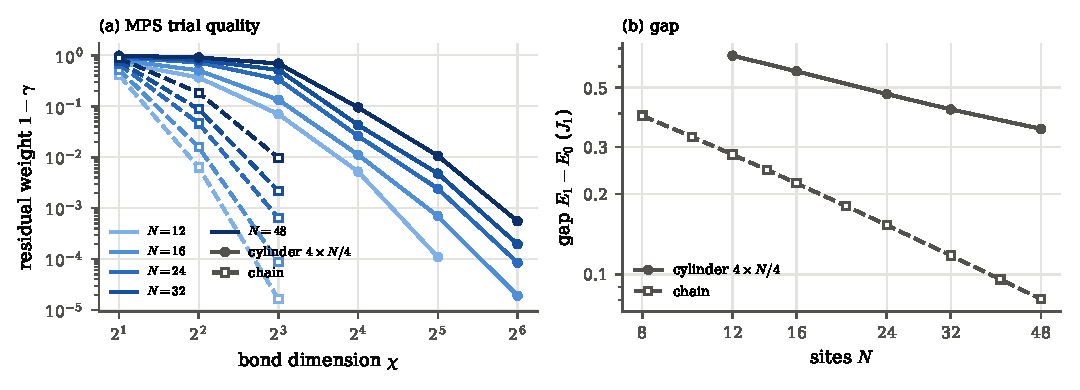
\includegraphics[width=\textwidth]{figs/fig_motivation_meas.pdf}
\caption{Chains (open squares, dashed) and $4\times N/4$ cylinders (filled circles, solid) at $J_2=0$, from DMRG
(verified against ED for $N\le16$). (a) Residual weight $1-\gamma$ of the optimal MPS against its bond dimension;
colors mark the number of sites. Chain trials were computed up to $\chi=8$. (b) Gap $E_1-E_0$ against $N$. Sources:
\texttt{results/inputs.json}, \texttt{results/ext\_inputs2d.json}.}
\label{fig:motivation}
\end{figure*}

%=====================================================================================================
\section{Gap and overlap as independent inputs}
\label{sec:gapov}

Along any natural family of chains the gap and the overlap move together: at fixed $J_2$ the gap closes with $N$, and
at fixed bond dimension the overlap decays with $N$. We therefore construct a family in which they are set
independently at every $N$.

\emph{Construction.} For each $N\in\{8,10,12,14\}$ and target gap $\Delta\in\{0.30,0.35,\dots,0.55\}$, $J_2$ is found
by bisection on exact diagonalization so that the singlet--triplet gap equals $\Delta$ to $10^{-9}$; pairs without a
solution below the dimerized regime are left out. For all tuned couplings the lowest $S^z=0$ excitation coincides
with the lowest triplet to $10^{-7}$, so $\Delta$ is the true gap. The trial is the variational $\chi=16$ MPS, prepared by
its staircase circuit, followed by $R_y(\theta)$ on every even site; rotating one sublattice breaks the singlet
symmetry and lowers $\gamma$ smoothly, and $\theta$ is set by bisection to hit the target $\gamma$. The trial circuit
is therefore the same along an overlap scan. Study A fixes $\Delta\in\{0.40,0.50\}$ and scans
$\gamma\in\{0.03,0.1,0.3,0.5,0.7,0.9\}$; study B fixes $\gamma\in\{0.1,0.5\}$ and scans $\Delta$; both at
$\epsilon\in\{10^{-2},10^{-3},10^{-4}\}$, \goNcases{} cases in all, each with the dyadic and optimized schedules and
with QETU (Sec.~\ref{sec:qetu}). Costs are for the filter alone unless stated.

\subsection{The gap sets the circuit, the overlap sets the repetitions}

Figures~\ref{fig:filterA} and~\ref{fig:filterB} show CNOTs, $R_z$ rotations and evolution time per shot, and CNOTs per
success, along both scans.

\emph{Per shot, the overlap enters only logarithmically.} At fixed gap, lowering $\gamma$ thirtyfold (0.9 to 0.03)
raises the CNOTs per shot of the dyadic filter by only \fAMDcnot$\times$ and its evolution time by \fAMDtime$\times$.
The filter must reach $\eta^2=\gamma\epsilon/(1-\gamma)$, and a worse trial adds only $\ln290\approx5.7$ to
$L=\ln[(1-\gamma)/(\gamma\epsilon)]$, already 2--13 here. The dyadic filter grows in whole pulses, so its per-shot cost
moves in steps.

\emph{Per shot, the gap enters as a power.} At fixed overlap, closing the gap by $1.8\times$ (0.55 to 0.30) raises the
CNOTs per shot by \fBMDcnot$\times$ and the evolution time by \fBMDtime$\times$. The evolution time follows the
textbook $T=O(\Delta^{-1}\ln\eta^{-1})$~\cite{Lin2020,Ge2019} (fitted exponent \fitMDTgap); the CNOTs per shot grow
faster, as $\Delta^{-\ciDShotgap}$ (Table~\ref{tab:gofit}), because a filter for a smaller gap also needs a finer Trotter
step (Sec.~\ref{sec:mech}), and $1.8^{\ciDShotgap}\approx3$ matches the observed \fBMDcnot$\times$.

\emph{Per success, the overlap returns as $1/\gamma$.} Every run succeeds with probability $p\approx\gamma F(0)^2$,
with $F(0)=1$ for the dyadic filter, so the cost per success carries $1/\gamma$. The gap decides the depth of the
coherent circuit, and with it whether the filter fits a coherence or error budget at all; the overlap decides how
often that circuit has to be run.

\emph{$R_z$ counts follow CNOT counts.} Each bond block has 3 $R_z$ and 6 CNOTs and each pulse adds one rotation, so
$R_z/\mathrm{CNOT}=\fRzCnot$ throughout, and every statement about CNOTs holds for the arbitrary rotations, and so for
the $T$ count of a fault-tolerant implementation up to the synthesis factor.

\begin{figure*}[t]
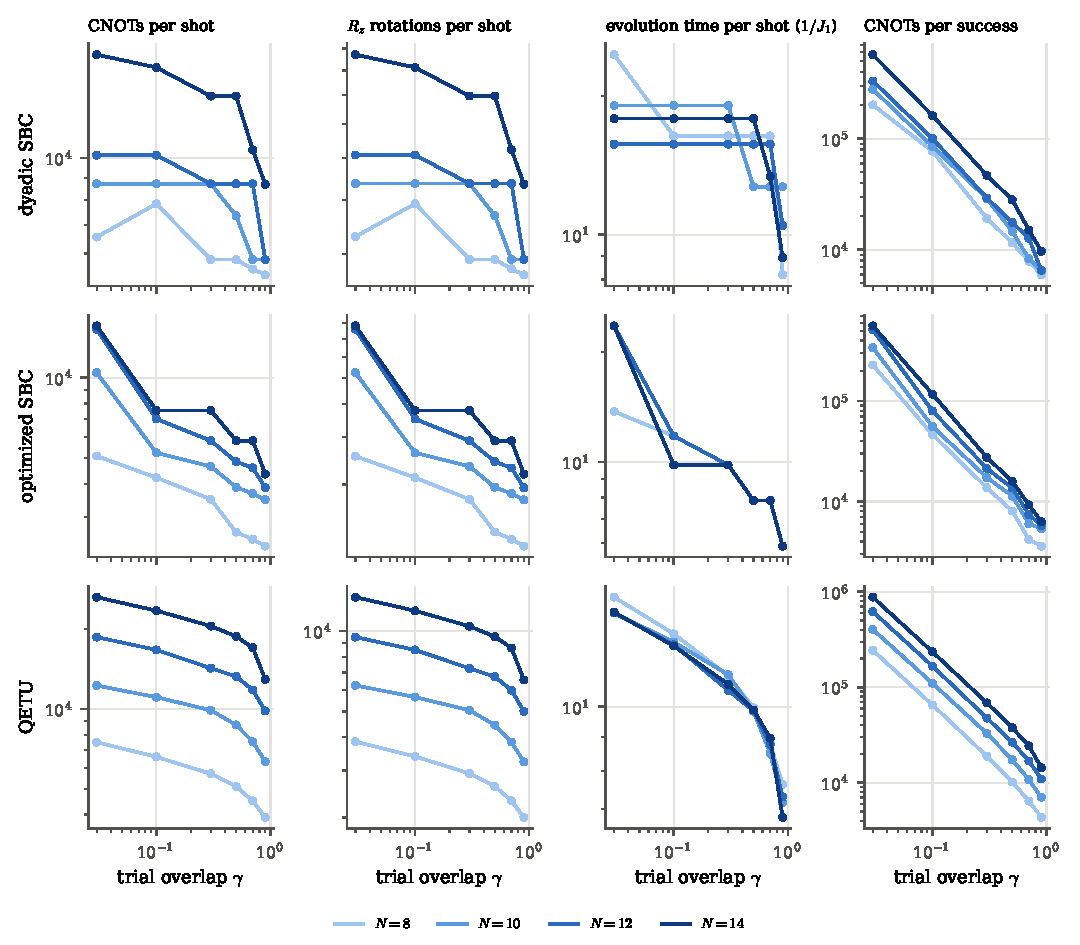
\includegraphics[width=\textwidth]{figs/fig_filter_A_meas.pdf}
\caption{Study A: filter-only resources at a gap held at $\Delta=0.40$ for every $N$, $\epsilon=10^{-3}$, against the trial overlap, measured by exact simulation. Rows: dyadic SBC, optimized SBC, QETU (Sec.~\ref{sec:qetu}). Columns 1--3 per shot, column 4 per success. Source: \texttt{results/gapov.jsonl}, \texttt{results/gapov\_filter.json}.}
\label{fig:filterA}
\end{figure*}

\begin{figure*}[t]
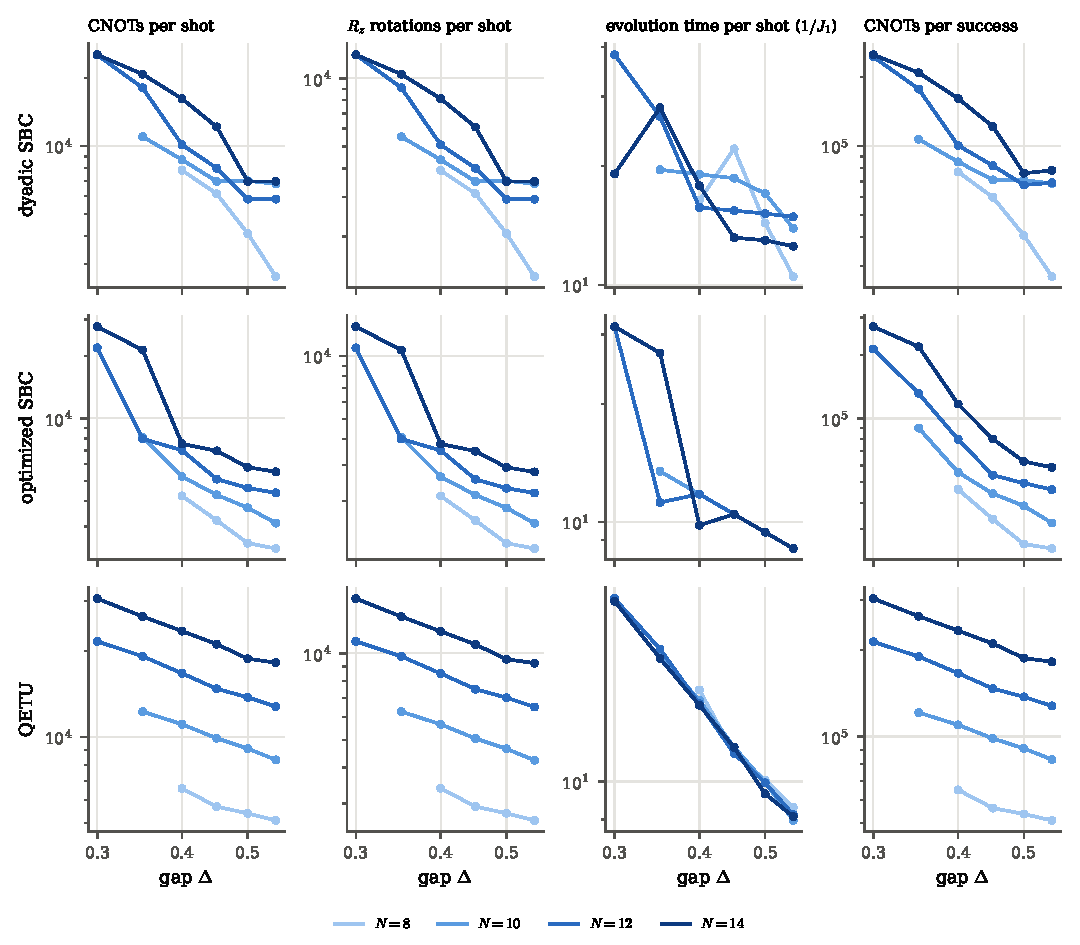
\includegraphics[width=\textwidth]{figs/fig_filter_B_meas.pdf}
\caption{Study B: as Fig.~\ref{fig:filterA} at an overlap held at $\gamma=0.10$ for every $N$, against the gap (held fixed across $N$ by tuning $J_2$).}
\label{fig:filterB}
\end{figure*}

\subsection{Cost laws with confidence intervals}

We fit three costs to
\begin{equation}
C\approx a\,N^{\alpha}\,\Delta^{-\beta}\,\big[\ln(1/\epsilon)\big]^{\lambda}\,\gamma^{-\nu}
\label{eq:fit}
\end{equation}
over all \goNcases{} cases: the filter's CNOTs per shot, its CNOTs per success, and the expected CNOTs per success of
the whole circuit (filter and trial). The target enters as $\ln(1/\epsilon)$, separately from the overlap, so that
$\nu$ measures the overlap alone. The 95\% intervals in Table~\ref{tab:gofit} come from a bootstrap that resamples the
\ciNsys{} $(N,\Delta)$ systems, not the individual cases, since cases on one system share a Hamiltonian.

The table states the paper's main result with error bars. For the dyadic filter, per shot,
\begin{equation}
C_{\rm shot}\propto N^{\ciDShotN}\,\Delta^{-\ciDShotgap}\,\big[\ln(1/\epsilon)\big]^{\ciDShoteps}\,\gamma^{-\ciDShotgam},
\end{equation}
with $\beta\in[\ciDShotgaplo,\ciDShotgaphi]$ and $\nu\in[\ciDShotgamlo,\ciDShotgamhi]$: the gap sets the circuit
and the overlap barely enters it. Per success the overlap exponent becomes $\nu=\ciDSuccgam$
$[\ciDSuccgamlo,\ciDSuccgamhi]$, the $1/\gamma$ of repeat-until-success, and the gap exponent stays at
\ciDSuccgap. The optimized and Chebyshev filters show the same split. With the trial circuit included, a cost that does
not depend on the gap, the gap exponent of the total falls to \ciDTotgap{} $[\ciDTotgaplo,\ciDTotgaphi]$, which is why
it is smaller than the per-shot value. Folding $\epsilon$ and $\gamma$ into $L=\ln[(1-\gamma)/(\gamma\epsilon)]$, as
the textbook bound does, gives an overlap exponent of \goMDgam{} for the total cost, but only because $L$ absorbs part
of the $1/\gamma$; fitted separately, as here, the overlap exponent is consistent with 1. These exponents summarize
$N=8$--14 and $\Delta=0.30$--0.55 and are not asymptotic laws. Appendix~\ref{app:dyaopt} compares the two SBC
schedules and maps the cost over the $(\Delta,\gamma)$ plane and over $(N,\epsilon)$.

\begin{table*}[t]
\caption{Fits of the measured costs to Eq.~\eqref{eq:fit} over all \goNcases{} gap/overlap cases, with 95\% intervals
from a bootstrap over the \ciNsys{} $(N,\Delta)$ systems. ``rms'': typical factor between a case and its fit. Source:
\texttt{results/gapov.jsonl}; \texttt{make\_review.py}.}
\label{tab:gofit}
\begin{ruledtabular}
\begin{tabular}{llrrrrrr}
filter & cost & $a$ & $\alpha$ ($N$) & $\beta$ ($\Delta^{-1}$) & $\lambda$ ($\ln\epsilon^{-1}$) & $\nu$ ($\gamma^{-1}$) & rms\\
\midrule
dyadic & filter, per shot & $5.6\times10^{-1}$ & $1.31_{[1.12,\,1.49]}$ & $1.91_{[1.60,\,2.16]}$ & $2.40_{[2.22,\,2.57]}$ & $0.14_{[0.12,\,0.16]}$ & 1.24 \\
dyadic & filter, per success & $6.4\times10^{-1}$ & $1.42_{[1.23,\,1.61]}$ & $1.72_{[1.43,\,1.96]}$ & $2.29_{[2.10,\,2.47]}$ & $1.14_{[1.11,\,1.16]}$ & 1.25 \\
dyadic & filter + trial, per success & $5.3$ & $1.52_{[1.37,\,1.66]}$ & $1.19_{[0.99,\,1.37]}$ & $1.54_{[1.36,\,1.70]}$ & $1.08_{[1.07,\,1.10]}$ & 1.19 \\
\addlinespace
optimized & filter, per shot & $1.6\times10^{-1}$ & $1.52_{[1.30,\,1.71]}$ & $1.86_{[1.58,\,2.07]}$ & $2.52_{[2.37,\,2.68]}$ & $0.27_{[0.25,\,0.28]}$ & 1.26 \\
optimized & filter, per success & $2.5\times10^{-1}$ & $1.45_{[1.27,\,1.63]}$ & $2.01_{[1.76,\,2.19]}$ & $2.44_{[2.29,\,2.60]}$ & $1.20_{[1.18,\,1.21]}$ & 1.23 \\
optimized & filter + trial, per success & $4.6$ & $1.52_{[1.41,\,1.64]}$ & $1.39_{[1.23,\,1.52]}$ & $1.46_{[1.32,\,1.62]}$ & $1.09_{[1.09,\,1.10]}$ & 1.20 \\
\addlinespace
QETU & filter, per shot & $3.2$ & $2.24_{[2.11,\,2.32]}$ & $0.99_{[0.87,\,1.08]}$ & $0.88_{[0.85,\,0.90]}$ & $0.18_{[0.18,\,0.19]}$ & 1.12 \\
QETU & filter, per success & $3.0$ & $2.24_{[2.12,\,2.33]}$ & $0.98_{[0.86,\,1.07]}$ & $0.89_{[0.87,\,0.92]}$ & $1.18_{[1.17,\,1.19]}$ & 1.12 \\
QETU & filter + trial, per success & $1.1\times10^{1}$ & $2.10_{[2.00,\,2.17]}$ & $0.76_{[0.66,\,0.84]}$ & $0.68_{[0.66,\,0.69]}$ & $1.14_{[1.13,\,1.14]}$ & 1.08 \\

\end{tabular}
\end{ruledtabular}
\end{table*}

\subsection{A second way to lower the overlap}
\label{sec:trunc}

The rotation lowers the overlap by spin flips, which put the missing weight mostly at high energy: the residual
of a rotation trial has a mean excitation energy of \rotResLo--\rotResHi{} gaps. To check that the split between gap
and overlap is not specific to that kind of residual, we repeat study A with a different mechanism. The trial is the
exact ground state truncated to Schmidt rank one on a chosen set of bonds (at most five), an MPS of bond dimension at
most 16 costed like the $\chi=16$ trial, whose error is an entanglement truncation and whose residual sits low in the
spectrum, \trResLo--\trResHi{} gaps above $E_0$. For each $N$, $\Delta\in\{0.40,0.50\}$ and target $\gamma$ the bond
set whose overlap lies closest to the target is used, giving $\gamma=\trGamLo$--\trGamHi{} (\trNcases{} cases with
$1-\gamma>\epsilon$; \texttt{run\_review.py trunc}).

The same law holds. Fitting Eq.~\eqref{eq:fit} to the truncation trials gives, for the dyadic filter, a per-shot
overlap exponent $\nu=\trDShotgam$ $[\trDShotgamlo,\trDShotgamhi]$ and a per-success exponent \trDSuccgam{}
$[\trDSuccgamlo,\trDSuccgamhi]$, against \ciDShotgam{} and \ciDSuccgam{} for the rotation trials, with
$\lambda=\trDShoteps$ for the target. (The gap exponent is poorly constrained here, since only two gaps are used.)
Predicting each truncation case's per-shot CNOTs from the rotation-trial fit of Table~\ref{tab:gofit} is off by a
median factor \trPredMed{} (range \trPredLo--\trPredHi). The overlap therefore enters through its size, not through
where in the spectrum the missing weight sits: the filter has to suppress every level above the gap, wherever the
weight is.


\subsection{Mechanism: filter length, Trotter step and gates per step}
\label{sec:mech}

The per-shot cost factorizes as
\begin{equation}
\text{CNOTs per shot}=\frac{T}{\delta t}\times c_{\rm step}(N),
\label{eq:factor}
\end{equation}
and each factor answers to different inputs (Fig.~\ref{fig:mech}).

\emph{Filter length.} The physical evolution time depends on the gap and $L$ only: a fit gives
$T\propto\Delta^{-\fitMDTgap}L^{\fitMDTL}N^{\fitMDTN}$ for the dyadic filter, so at fixed absolute gap the filter length
does not depend on the size of the system.

\emph{Trotter step.} The filter tolerates very coarse steps: median $\delta t=\fDtDTwo$, \fDtDThree, \fDtDFour{} (in
$1/J_1$) at $\epsilon=10^{-2}$, $10^{-3}$, $10^{-4}$, larger at larger gap. The step shrinks roughly as
$\epsilon^{0.3}$ and as $\Delta^{0.7}$ (steps per shot grow as $\Delta^{-\fitMDSgap}$ against $\Delta^{-\fitMDTgap}$
for the time), and barely depends on $N$, so the number of steps per shot grows as $L^{\fitMDSL}$ and $N^{\fitMDSN}$.
The bisection assumes that a circuit which passes at some step also passes at every finer one.
We checked this on \monoCases{} cases ($N=8$ and 10; three overlaps at $\Delta=0.40$ and three gaps at
$\gamma=0.1$; all three targets) by scanning the common step on a dense logarithmic grid from one step per pulse down
to an eighth of the bisected step. For the dyadic filter and for QETU (one to six steps per query) passing was
monotone in every scan: once a step passes, every finer step passes. The exceptions are all in the optimized SBC
filter, \monoOK{} of \monoN{} SBC scans being monotone. Its pulse times are unequal, so the number of steps in each
pulse is rounded separately and the realized error does not fall smoothly with the step. In four of the six exceptions
the failing step lies above the bisected one, which only means the bisection could have stopped at a coarser step
(the dense scan found a passing step up to \monoRatioHi{} times coarser; median ratio \monoRatioMed). In two
($N=8$ and 10 at $\Delta=0.30$) a step finer than the bisected one fails, at 0.72 and 0.91 times it, with infidelity
up to \monoWorst{}$\,\epsilon$. The step we report is always one that was evaluated and passed, so the tables are
unaffected, but for the optimized filter a finer step is not automatically safe and the chosen step must be checked
directly.


\emph{Measured step against the bounds.} Figure~\ref{fig:bounds} sets each measured step beside two bounds evaluated
for the same filter and target, with half of $\sqrt\epsilon$ allotted to Trotter error: the worst-case commutator
bound for Strang steps (exact local norms of the nested commutators~\cite{Childs2021}) and the explicit low-energy
bound of Mizuta and Kuwahara~\cite{Mizuta2025} (their Corollary S4), evaluated in its most favorable case, for a state
inside the ground space. The measured dyadic step is a median \bdCommMed{} times the commutator step (range
\bdCommLo--\bdCommHi; \bdCommOptimizedMed{} for the optimized filter, \bdCommQetuMed{} for QETU, whose short queries
leave less room). The low-energy bound, which improves on Şahinoğlu and Somma~\cite{Sahinoglu2021}, scales better with
the energy but does worse here: the ground state of a frustrated antiferromagnet lies an extensive energy above the
zero of the positive-semidefinite bond terms that the bound measures from, and its constants restrict it to
$\delta t\le\bdMKvalid/J_1$, so it asks for steps \bdMKMed{} times finer than measured. Its asymptotic advantage does
not reach these sizes. The pulses are long and smooth, the filtered state sits at the bottom of the spectrum, and the
Trotter error that matters is the error on that state, which neither bound resolves.

\emph{Gates per step.} One Strang step costs a median $\fCps\,N$ CNOTs for the two-neighbor chain ($6(2B-2)$ with
$B=2N-3$ bonds). With a step count nearly independent of $N$, the CNOTs per shot grow as $N^{\ciDShotN}$, almost
entirely through the gates per step.

\begin{figure*}[t]
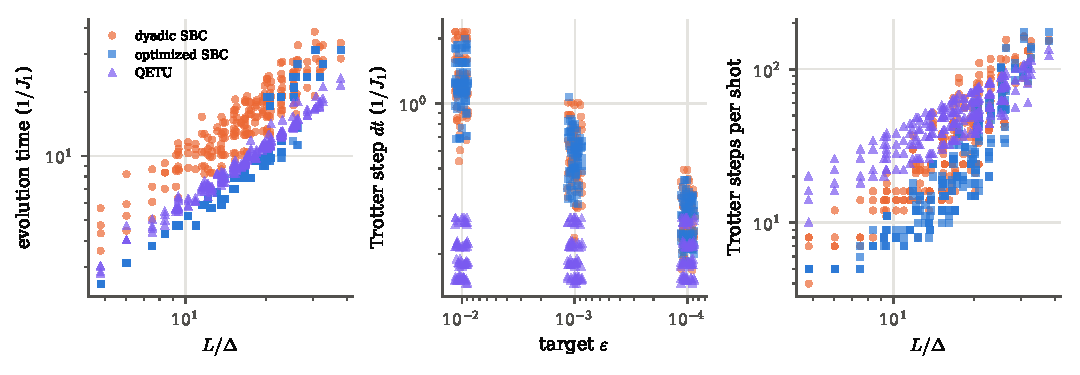
\includegraphics[width=\textwidth]{figs/fig_filter_mech_meas.pdf}
\caption{All \goNcases{} cases, measured. (a) Evolution time against $L/\Delta$, $L=\ln[(1-\gamma)/(\gamma\epsilon)]$. (b) Coarsest passing Trotter step against $\epsilon$ (jittered horizontally). (c) Trotter steps per shot against $L/\Delta$. Orange circles: dyadic SBC; blue squares: optimized SBC; purple triangles: QETU.}
\label{fig:mech}
\end{figure*}

\begin{figure}[t]
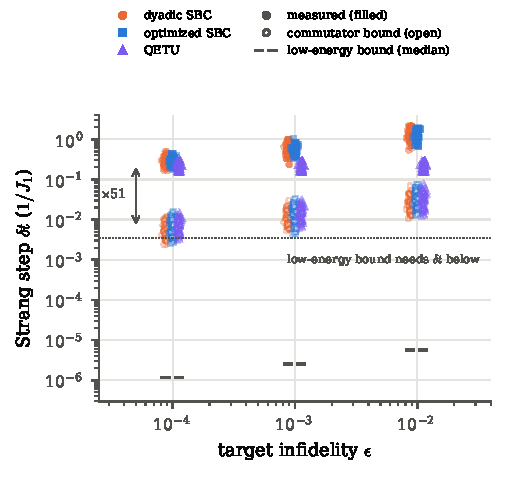
\includegraphics[width=\columnwidth]{figs/fig_bounds_rev.pdf}
\caption{Coarsest passing Strang step in the controlled study (filled) against the commutator bound for the same filter
and target (open), and the median low-energy bound of Ref.~\cite{Mizuta2025} (dashed), which holds only below the dotted
line. Source: \texttt{results/review\_bounds.json}.}
\label{fig:bounds}
\end{figure}

%=====================================================================================================
\section{Comparison with a Chebyshev filter (QETU)}
\label{sec:qetu}

QETU~\cite{Dong2022} uses $d$ queries of $e^{-i\tau H_s\otimes Z_a}$ interleaved with ancilla rotations and a single
post-selection, so that the ancilla-0 block is $p(\cos\tau H_s)$ for a real even polynomial $p$ of degree $d$ with
$|p|\le1$. With the stop band mapped to $[0,x_s]$, $x_s=\cos(\tau\delta)$, we take the extremal Chebyshev filter
\begin{equation}
p(x)=\frac{T_d(x/x_s)}{T_d(1/x_s)},
\end{equation}
which has $p$ equal to 1 at the ground state and needs $T=d\tau\approx\delta^{-1}\ln(2/\eta)$, two to three times less
evolution than the dyadic ladder. Each query is Trotterized like an SBC pulse and costed in the same controlled form
(Sec.~\ref{sec:pipeline}); the classical phase-finding step costs no quantum gates and is not counted. By simulation
on exact spectra for $N=8$--16 (\empN{} cases), the smallest degree that reaches $\epsilon$ is set by the gap and the
target alone, $d_{\min}\delta\simeq(2/\pi)\cosh^{-1}(1/\eta)$, whatever the shape of the trial's excited weight,
because the Chebyshev filter suppresses every level above the gap equally.

\emph{Query length $\pi/2$.} With $\tau=\pi/2$, the choice of Dong, Lin and Tong~\cite{Dong2022}, QETU is cheaper than
the dyadic filter in \goQetuWinsTwo{} of \goCasesTwo{} cases at $\epsilon=10^{-2}$, \goQetuWinsThree{} of
\goCasesThree{} at $10^{-3}$ and \goQetuWinsFour{} of \goCasesFour{} at $10^{-4}$. The reason is the Trotter step, not
the filter: QETU needs less evolution time (median \fQDtime$\times$ dyadic), but one Strang step per short query,
$\delta t=\tau/W\propto1/N$, so its step count is a median \fQDsteps$\times$ the dyadic one and its CNOTs grow as
$N^{\fitMQCN}$ against $N^{\fitMDCN}$. The long dyadic pulses tolerate steps of order $1/J_1$, but these shrink as
roughly $\epsilon^{0.3}$, and by $\epsilon=10^{-4}$ the shorter filter wins.

\emph{Longest admissible query.} Any $\tau\le\pi/(1+\delta)$ keeps every excited level inside
$|\cos\tau E|\le\cos\tau\delta$, and one Strang step per query still suffices at longer queries. Redoing every QETU
search at $\tau=3\pi/4$ and $\pi/(1+\delta)$ (\tauNcases{} cases: the \tauNgo{} controlled cases and the \tauNact{} cases of Sec.~\ref{sec:crossover}) lowers its cost to a median \tauPiMed{} (range
\tauPiMin--\tauPiMax) of the $\tau=\pi/2$ cost at $\tau=\pi/(1+\delta)$. With QETU at its best $\tau$
(Table~\ref{tab:qetutau}) the SBC filters keep $\epsilon=10^{-2}$ (QETU cheapest in \tauBestQeTwo{} of 74), the two
families split $10^{-3}$ (\tauBestQeThree{} of 74), and QETU is the cheapest filter in \tauBestQeFour{} of 74 at
$10^{-4}$. The fair statement is that SBC wins at loose targets, the two are even at $10^{-3}$, and the Chebyshev
filter wins from $10^{-4}$ on.

\begin{table}[t]
\caption{Cheapest measured filter in the controlled study (74 cases per target; dyadic/optimized/QETU) with QETU at
$\tau=\pi/2$ and at its best query length $\tau\in\{\pi/2,3\pi/4,\pi/(1+\delta)\}$. Source:
\texttt{results/qetu\_tau.jsonl}.}
\label{tab:qetutau}
\begin{ruledtabular}
\begin{tabular}{lll}
target & $\tau=\pi/2$ & best $\tau$\\
\midrule
$\epsilon=1\times10^{-2}$ & 23/51/0 & 19/48/7 \\
$\epsilon=1\times10^{-3}$ & 16/57/1 & 4/32/38 \\
$\epsilon=1\times10^{-4}$ & 5/32/37 & 0/9/65 \\

\end{tabular}
\end{ruledtabular}
\end{table}

%=====================================================================================================
\section{Benchmark against the MPS alone}
\label{sec:crossover}

The alternative to filtering a cheap trial is compiling a better MPS. We compare the two at equal target infidelity:
for each system every MPS trial with $\chi=2,\dots,64$ is decomposed on the exact spectrum, and for each
$\epsilon\in[10^{-5},10^{-2}]$ the cheapest route is found, the smallest MPS that meets $1-\gamma\le\epsilon$ alone,
against the cheapest smaller MPS followed by a measured SBC or QETU filter, with cost (trial $+$ filter)$/p$. Both
routes use the staircase MPS cost of Sec.~\ref{sec:pipeline}.

\emph{Chains.} On nine chains ($N=12$, 14, 16 at $J_2=0$, 0.2411, 0.4; Fig.~\ref{fig:actual1d}) compiling the MPS is
cheaper in most cases: the filtered route wins \actOneWins{} of \actOneTot{} targets, by 1.1--\actOneRatioMax$\times$.
Every win filters a trial that misses the target by $(1-\gamma)/\epsilon\le\actOneFarMax$, with a dyadic ladder of
one to four pulses (1--21 Strang steps, $p\ge0.988$), and all \actOneFar{} candidate routes with a larger ratio lose,
by a median \actOneFarMed$\times$. The filter acts as a last-mile polisher: MPS cost jumps about fourfold per doubling
of $\chi$, so a target just below what a given $\chi$ reaches forces the MPS-alone route up a bond dimension, while a
short filter removes the small residual of the lower one. The wins are therefore tied to the bond-dimension grid
rather than to $N$ or $J_2$. The optimized design never wins, because suppression over the whole band above $\delta$
needs $T\gtrsim\pi/\delta$ (scaled) where one dyadic pulse suffices, and QETU beats the MPS alone at 11 targets but is never the
cheapest route.

\emph{Cylinders.} On the $4\times3$ and $4\times4$ cylinders at $J_2=0$ and 0.3 (Fig.~\ref{fig:actual}), the picture
reverses, as Fig.~\ref{fig:motivation} anticipates. A snake MPS struggles here: at
$4\times4$, $J_2=0$, $\chi=16$ misses $\epsilon=10^{-2}$ ($1-\gamma=1.1\times10^{-2}$), $\chi=32$ stalls at
$7\times10^{-4}$ and no $\chi\le64$ reaches $10^{-5}$, while the compile cost grows about fourfold per doubling (5\,328,
20\,548 and 76\,600 CNOTs for $\chi=16$, 32, 64). The filtered route is cheaper at 27 of the 28 cylinder targets, by
1.1--\actRatioMax$\times$, and is the only MPS-based route at $10^{-5}$ on $4\times4$. Every win uses the dyadic ladder,
mostly on a $\chi=16$ trial, with $p\ge0.77$ and 1--46 Strang steps, and recovers factors $(1-\gamma)/\epsilon$ up to
$10^3$. The filter's depth grows only as $\ln(1/\epsilon)$ at fixed gap, while the MPS needed to reach $\epsilon$ alone
grows fourfold per bond-dimension step. All trials are snake MPS, a weak choice in two dimensions, and the staircase
cost charges every site a unitary on $b+1$ qubits even where the bond is smaller, which favors the filtered route most
where its trial is cheap.

\emph{Harder baselines.} Two changes to the accounting test whether this conclusion rests on a weak baseline. First,
an MPS staircase is a sequence of isometries rather than unitaries, and isometry decompositions save part of the
quantum Shannon count~\cite{Iten2016}; charging every staircase unitary, in both routes, at half its quantum Shannon
count leaves the filtered route cheaper at \blChainWinsHalf{} of \blChainTot{} chain targets (from \blChainWins) and
\blCylWinsHalf{} of \blCylTot{} cylinder targets (from \blCylWins). Second, at these sizes the exact ground state is
known, and generic state preparation~\cite{Plesch2011} reaches any target at a fixed cost of
\genPrepTwelve, \genPrepFourteen{} and \genPrepSixteen{} CNOTs for 12, 14 and 16 qubits. It never beats the cheaper
of the other two routes on chains. On the 12-site $4\times3$ cylinders it does, at \blCylGen{} of their 14 targets
($\epsilon\le3\times10^{-3}$), but already at 16 sites its cost exceeds every filtered route. Generic preparation needs
the full state vector and grows as $2^N$, so it is a ceiling only where exact diagonalization is possible; it shows
that on the smallest cylinders the filtered route wins against the MPS, not against every alternative. A non-snake trial, a product of exact
ground states of 4-site rings or 8-site blocks, and cylinders up to $4\times6$ are part of the larger runs described
in Sec.~\ref{sec:discussion}.

\begin{figure*}[t]
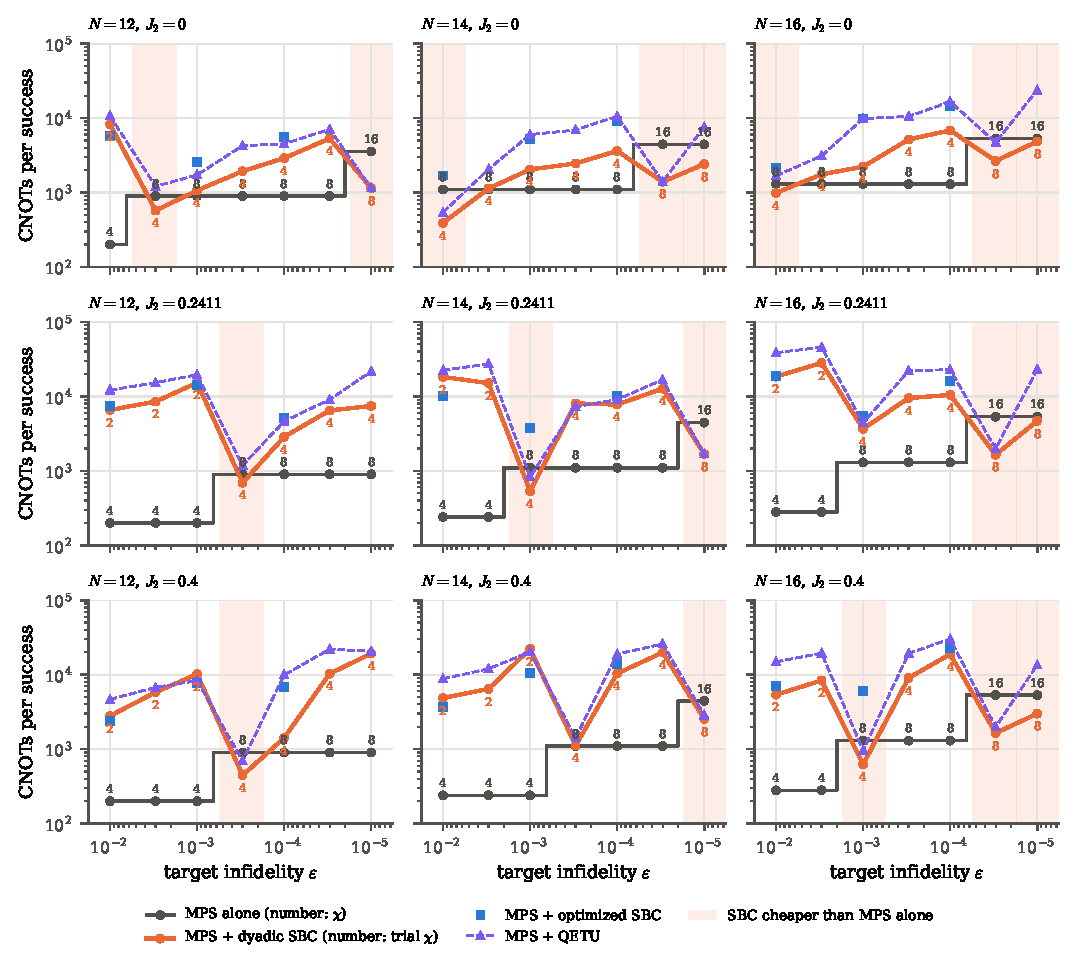
\includegraphics[width=\textwidth]{figs/fig_actual1d.pdf}
\caption{Measured cheapest route to infidelity $\epsilon$ on chains of $N=12$, 14, 16 (columns) at $J_2=0$,
0.2411, 0.4 (rows), all by exact simulation. Grey: cheapest MPS that meets $1-\gamma\le\epsilon$ alone (number:
$\chi$). Orange: cheapest smaller MPS followed by the dyadic SBC filter (number: trial $\chi$); blue squares:
optimized SBC (designed at $\epsilon=10^{-2},10^{-3},10^{-4}$ only); purple: QETU. Shaded: the SBC route is
cheaper. Cost is (trial $+$ filter CNOTs)$/p$. Sources: \texttt{results/emp\_actual1d.jsonl} and, for
$N=16$, $J_2=0.2411$, \texttt{results/emp\_actual.json}.}
\label{fig:actual1d}
\end{figure*}

\begin{figure*}[t]
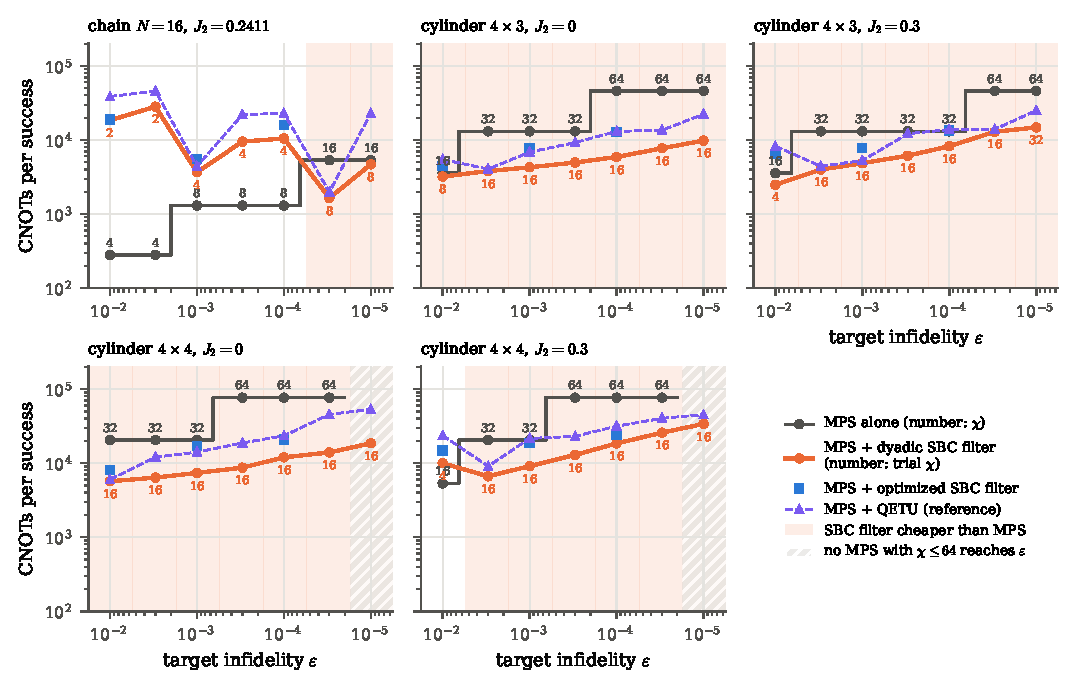
\includegraphics[width=\textwidth]{figs/fig_actual.pdf}
\caption{Measured cheapest route to infidelity $\epsilon$ on the 16-site chain and on small cylinders. Grey:
the cheapest MPS that meets the target alone (number: $\chi$). Orange: the cheapest smaller MPS followed
by the dyadic SBC filter (number: trial $\chi$); blue squares: optimized SBC; purple: QETU. Shaded:
the filtered route is cheaper; hatched: no MPS with $\chi\le64$ reaches $\epsilon$. Every cost is (trial $+$
filter CNOTs)$/p$ from exact simulation. Source: \texttt{results/emp\_actual.json}.}
\label{fig:actual}
\end{figure*}

%=====================================================================================================
\section{Planning from DMRG alone, verified against exact diagonalization}
\label{sec:dmrg}

The benchmarks above pick the filter and the Trotter step with the exact ground state. Here we run the workflow as an
experiment would, from DMRG alone, on systems small enough that exact diagonalization (ED) checks the outcome at the
end. The workflow has two classical ingredients with different roles. A large-bond-dimension DMRG run ($\chi\le256$)
converges the energies to machine level: it reproduces the ED values of $E_0$ and $E_1$ (the lowest $S^z=1$ state) to
$\dmrgEzeroErr$ and $\dmrgEoneErr$ at every size checked, and it provides a reference MPS. The trial that is compiled
into the circuit is a much smaller MPS, cheap enough to prepare, and its overlap $\gamma$ with the reference MPS, which
agrees with its overlap with the ED ground state to $\dmrgGammaErr$, is what falls short of the target. The energies
place the filter's window; the overlap is the reason a filter is needed and sets how much it must suppress.

\emph{End to end.} For every chain ($N=12$, 14, 16) and cylinder ($4\times3$, $4\times4$) target of
Sec.~\ref{sec:crossover}, $\epsilon=10^{-5}$--$10^{-2}$, with the SBC (dyadic or optimized) and QETU filters (\apN{}
cases; \texttt{run\_aposteriori.py}), the trial is the low-$\chi$ MPS ($\chi=2$--64) that leads to the cheapest
circuit. Its residual weight $1-\gamma$ ranges from $2\times10^{-5}$ to 0.4 and exceeds the target by a median factor
of 7. The filter is designed from the DMRG energies and the DMRG estimate of $\gamma$, and the Trotter step is chosen
without the ground state: starting from $\delta t=4/J_1$, halve it until the post-selected energy changes by at most
$\epsilon\Delta/2$ between successive steps, and keep the finer one. Because the leaked weight sits at least $\Delta$
above $E_0$, an infidelity $\epsilon$ moves the energy by at least $\epsilon\Delta$, so the rule errs on the safe side.
Checked against ED, the prepared state met the target in \apEok{} of \apEtot{} cases, at a median \apEorS{} (SBC) and
\apEorQ{} (QETU) times the cost with the coarsest step that passes. The price is the calibration: resolving
$\epsilon\Delta/2$ in the three measurement bases of the Heisenberg energy takes a median $\apShotsMed$ post-selected
shots per case, about $10^{7}$ at $\epsilon=10^{-2}$ and growing as $\epsilon^{-2}$, which pays off only if the circuit
is then reused many times.

\emph{Sensitivity to the inputs.} With converged DMRG the energies are not the limiting input, but a filter should
still fail gracefully if they are off, for example when DMRG is not converged on a harder system. We therefore perturbed
the inputs by hand for every $N\le14$, all three couplings and the dyadic, optimized and QETU filters at
$\epsilon=10^{-2}$, with a conservative Trotter step so that only the filter design is tested, and simulated each
circuit on the true trial state (Table~\ref{tab:senswide}). With exact inputs all \sensGapN{} filters meet the target.
Overestimating the gap moves the stop-band edge above the first excitation: by 10\% it breaks the target in
\sensGapOneTenMiss{} of \sensGapN{} cases (marginally, worst \sensGapOneTenWorst), by 25\% in
\sensGapOneQuarterMiss{} and by 50\% in \sensGapOneHalfMiss. The dyadic filter is the most tolerant
(\sensDyaQuarterMiss{} misses at 25\%), because its suppression is far below the target over most of the band; the
optimized and Chebyshev filters, designed to sit right at the target, have no slack. Underestimating the gap is safe and
cheap: assuming \gapMarginF{} of it costs \gapMarginCost$\times$. Overestimating $\gamma$ broke the target in
\sensGammaMiss{} of \sensGammaN{} cases, every one because the inflated overlap crossed $1-\epsilon$ and the pipeline
dropped the filter altogether. When DMRG is not converged, its error bars catch it: taking each energy's change between
the last two bond dimensions as its error, the intervals contained both exact energies in all \mgN{} tests on stopped
bond-dimension ladders (\texttt{run\_margin.py}), and the energy window became inconsistent, so that the pipeline
refused to plan, before the gap error grew large enough to matter.

\begin{table*}[t]
\caption{Gap and overlap overestimation for every $N\in\{8,10,12,14\}$ and $J_2$ (12 instances),
$\epsilon=10^{-2}$, second order: number of plans that miss the target and the worst measured
infidelity. $f$: assumed over true gap or $\gamma$. Source: \texttt{results/ext\_sensitivity.json}.}
\label{tab:senswide}
\begin{ruledtabular}
\begin{tabular}{lrrrrrrr}
 & & \multicolumn{2}{c}{dyadic} & \multicolumn{2}{c}{optimized} & \multicolumn{2}{c}{QETU}\\
input & $f$ & miss & worst & miss & worst & miss & worst\\
\midrule
gap & 1 & 0/12 & $1.7\times10^{-3}$ & 0/12 & $4.2\times10^{-3}$ & 0/12 & $2.3\times10^{-3}$ \\
gap & 1.1 & 0/12 & $6.5\times10^{-3}$ & 1/12 & $1.1\times10^{-2}$ & 1/12 & $1.0\times10^{-2}$ \\
gap & 1.25 & 0/12 & $6.8\times10^{-3}$ & 5/12 & $2.6\times10^{-2}$ & 5/12 & $3.0\times10^{-2}$ \\
gap & 1.5 & 2/12 & $6.3\times10^{-2}$ & 7/12 & $6.8\times10^{-2}$ & 7/12 & $9.2\times10^{-2}$ \\
gap & 2 & 8/12 & $1.4\times10^{-1}$ & 7/12 & $1.5\times10^{-1}$ & 11/12 & $2.2\times10^{-1}$ \\
gap & 3 & 11/12 & $2.2\times10^{-1}$ & 12/12 & $2.5\times10^{-1}$ & 12/12 & $3.1\times10^{-1}$ \\
$\gamma$ & 1.02 & 1/12 & $2.4\times10^{-2}$ & 1/12 & $2.4\times10^{-2}$ & 1/12 & $2.4\times10^{-2}$ \\
$\gamma$ & 1.05 & 3/12 & $5.5\times10^{-2}$ & 3/12 & $5.5\times10^{-2}$ & 3/12 & $5.5\times10^{-2}$ \\

\end{tabular}
\end{ruledtabular}
\end{table*}

%=====================================================================================================
\section{Discussion}
\label{sec:discussion}

\emph{What sets the cost.} The gap determines the coherent circuit: evolution time $\propto L/\Delta$, independent of
$N$ at fixed gap, and CNOTs and $R_z$ per shot that scale as a power of $1/\Delta$. The overlap enters the circuit only
through a logarithm and the expected cost through $1/\gamma$, so the filter tolerates a poor trial by paying in
repetitions rather than depth; amplitude amplification~\cite{Brassard2002,Yoder2014} would turn $1/\gamma$ into
$1/\sqrt\gamma$ at the price of a deeper coherent circuit, and is not modeled. The target enters through $L$ and,
because the tolerated Trotter step shrinks as $\epsilon^{0.3}$, through the step count.

\emph{Which filter.} The long, smooth SBC pulses tolerate Trotter steps of order $1/J_1$, which is why the cosine
filter wins at loose targets even though it needs more evolution time than a Chebyshev filter; from $\epsilon=10^{-4}$
the shorter Chebyshev filter wins. Among the SBC schedules the optimized design is cheaper in most cases (median
\odMMed$\times$ dyadic) but needs a nonconvex design that occasionally fails, while the dyadic ladder needs no design
at all.

\emph{When filtering pays.} A filter pays where the trial is hard to improve. For chains the MPS infidelity falls
quickly with $\chi$, so the filter helps only as a last-mile polisher; on small cylinders, where a snake MPS needs a
fast-growing bond dimension, it wins almost everywhere. DMRG on larger cylinders, up to $4\times12$, shows the
same two conditions growing stronger with size: the snake MPS gets worse at fixed $\chi$ while the gap stays above 0.35,
which makes two-dimensional systems the natural target for this workflow, beyond the sizes we could simulate.

\emph{Measured costs and what an experiment pays.} The benchmarks use the exact ground state to pick the shortest
sufficient filter and the coarsest sufficient Trotter step. Planned from DMRG alone, with the step set by energy
convergence, the filter met the target in every case we could check, at about twice the measured gate cost, but the
calibration costs $\epsilon^{-2}$ shots. Converged DMRG makes the energies essentially exact, and the
small trial MPS's overlap is what the filter has to repair. If the energies were off, the gap is the input to protect:
a 10--25\% overestimate breaks the optimized and Chebyshev filters, while an underestimate costs little. All of this was verified at sizes where ED is available; at larger
sizes the same workflow runs, but its outcome can no longer be checked.

\emph{Limitations.} Noiseless simulation; all-to-all connectivity; repeat-until-success rather than early abort; trial
circuits costed by a generic decomposition bound; and sizes ($N\le16$, 16-site cylinders) at which classical methods
are exact, so the fitted exponents are descriptive. The gap range that can be held fixed across $N$ (0.30--0.55) lies
in the easy regime, well above the gaps of longer natural chains.

\section*{Code and data availability}
The \texttt{sbpipe} package, the study scripts, all raw results and the sources of this paper are available at
\url{https://github.com/aaronseymour7/FilterPipeline}.

\appendix

\section{Dyadic versus optimized SBC, and cost maps}
\label{app:dyaopt}

The dyadic ladder has zero phases, so it passes the ground state with $F(0)=1$ and its length grows in whole pulses.
The optimized design is shorter, at the price of $F(0)<1$: its success probability is a median \optPgMed{} times
$\gamma$ (as low as \optPgLo). Per shot it uses a median \odShotTime{} times the dyadic evolution time and
\odShotSteps{} times its Trotter steps, at the same tolerated step. Per success it is a median \odMMed$\times$ the
dyadic cost (range \odMLo--\odMHi) and the cheaper one in \odMWins{} of \goNcases{} cases. Counting the cheapest of the
three filters case by case, the optimized SBC filter wins \bestOpTwo{} of \goCasesTwo{} cases at $\epsilon=10^{-2}$
(dyadic the other \bestDyTwo), \bestOpThree{} at $10^{-3}$ (dyadic \bestDyThree, QETU \bestQeThree), and \bestOpFour{}
at $10^{-4}$, where QETU takes \bestQeFour{} and dyadic \bestDyFour, all with QETU at $\tau=\pi/2$. The price of the
optimized schedule is its design: a nonconvex optimization of about 40\,s per case that had to be repeated with other
seeds in \optRetried{} of \optPoints{} points.

At fixed $N$ and $\epsilon=10^{-2}$ (Fig.~\ref{fig:gridmap}), the contours of the dyadic cost per success run nearly
parallel to the gap axis for $g\gtrsim0.40$: there the overlap alone sets the cost, from $2$--$6\times10^3$ CNOTs at
$\gamma=0.9$ to $1$--$4\times10^5$ at $\gamma=0.03$; below $g\approx0.40$ the gap starts to matter. The optimized
filter is cheaper over most of the map, and its contours tilt toward the gap axis, as its steeper gap exponent implies.
At fixed gap and overlap (Fig.~\ref{fig:heat}), the cost per success grows 7--21$\times$ (dyadic) from
$\epsilon=10^{-2}$ to $10^{-5}$ and 1.8--4.6$\times$ from $N=8$ to 14, so over this range the target matters more than
the size.

\begin{figure*}[t]
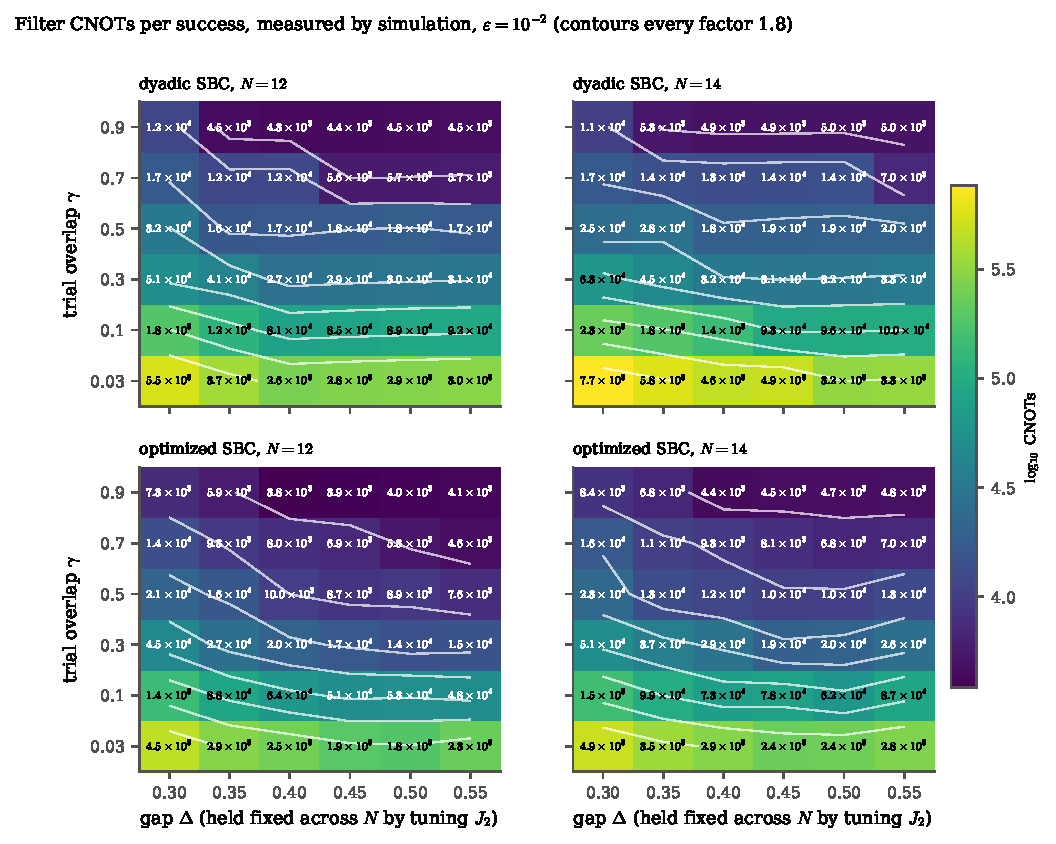
\includegraphics[width=0.85\textwidth]{figs/fig_gridmap.pdf}
\caption{Filter CNOTs per success over gap and overlap at $\epsilon=10^{-2}$, measured, for the dyadic
(top) and optimized (bottom) SBC filters at $N=12$ and 14. White contours every factor 1.8. Source:
\texttt{results/gapov.jsonl}, \texttt{results/gapov\_grid.jsonl}.}
\label{fig:gridmap}
\end{figure*}

\begin{figure*}[t]
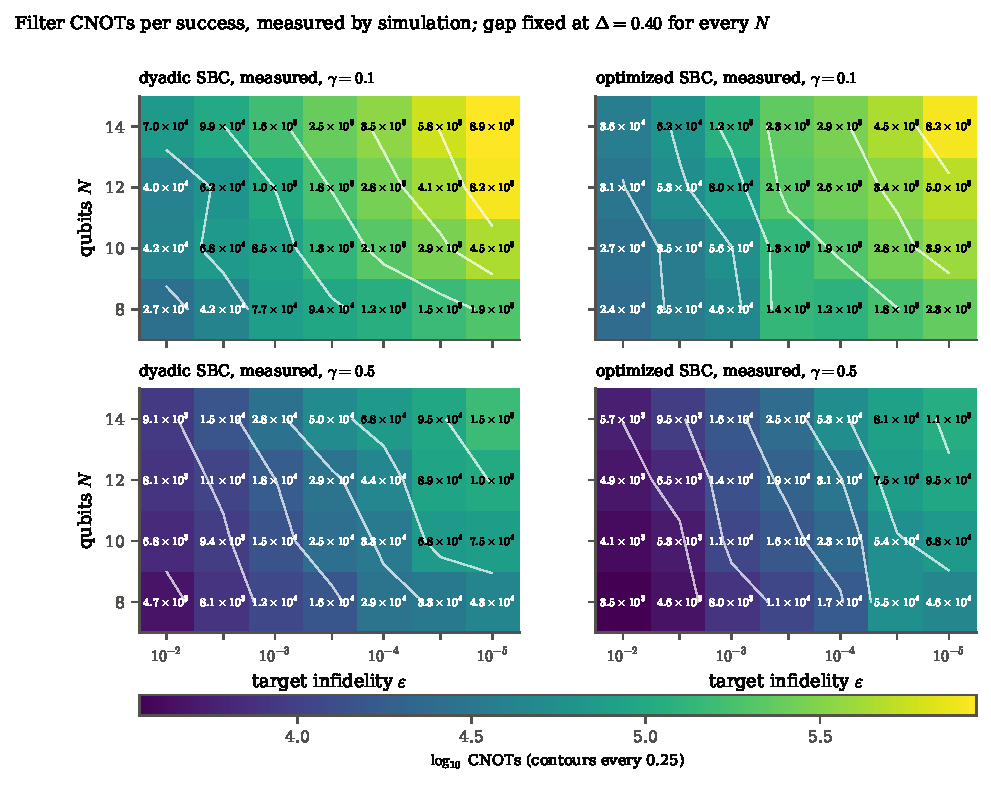
\includegraphics[width=0.85\textwidth]{figs/fig_heat_meas_succ.pdf}
\caption{Filter CNOTs per success over $N$ and $\epsilon$ at a gap held at $g=0.40$, measured, for the
dyadic (left) and optimized (right) SBC filters at $\gamma=0.1$ (top) and 0.5 (bottom). Source:
\texttt{results/gapov*.jsonl}.}
\label{fig:heat}
\end{figure*}

\section{Reproducing the results}
\label{app:repro}

The code, raw results and paper sources are at \url{https://github.com/aaronseymour7/FilterPipeline}. The controlled
study is run by \texttt{sbpipe\_study/run\_gapov.py} and summarized by \texttt{derive\_gapov\_filter.py}; the
benchmarks against the MPS alone and the QETU degree analysis by \texttt{run\_empirical.py}; the QETU query-length
study by \texttt{run\_qetu\_tau.py}; the DMRG-only runs by \texttt{run\_aposteriori.py}, the DMRG error-bar test by
\texttt{run\_margin.py}, and the wrong-input study by \texttt{run\_extended.py}. \texttt{make\_figures.py} writes the tables and numerical macros, and
\texttt{make\_figures\_measured.py} the measured-only figures and fit table used here. \texttt{python -m pytest
sbpipe/tests} checks the components, including the bond block of Eq.~\eqref{eq:bond} and the Dirichlet
identity~\eqref{eq:dirichlet}.

%=====================================================================================================
\begin{thebibliography}{99}
\bibitem{Stetcu2023} I.~Stetcu, A.~Baroni, and J.~Carlson, Projection algorithm for state preparation on
  quantum computers, Phys.\ Rev.\ C \textbf{108}, L031306 (2023), arXiv:2211.10545.
\bibitem{White1992} S.~R. White, Density matrix formulation for quantum renormalization groups,
  Phys.\ Rev.\ Lett.\ \textbf{69}, 2863 (1992).
\bibitem{Schollwock2011} U.~Schollw\"ock, The density-matrix renormalization group in the age of matrix
  product states, Ann.\ Phys.\ \textbf{326}, 96 (2011).
\bibitem{Ran2020} S.-J. Ran, Encoding of matrix product states into quantum circuits of one- and
  two-qubit gates, Phys.\ Rev.\ A \textbf{101}, 032310 (2020).
\bibitem{Ge2019} Y.~Ge, J.~Tura, and J.~I. Cirac, Faster ground state preparation and high-precision
  ground energy estimation with fewer qubits, J.\ Math.\ Phys.\ \textbf{60}, 022202 (2019).
\bibitem{Lin2020} L.~Lin and Y.~Tong, Near-optimal ground state preparation, Quantum \textbf{4}, 372
  (2020).
\bibitem{Gilyen2019} A.~Gily\'en, Y.~Su, G.~H. Low, and N.~Wiebe, Quantum singular value transformation
  and beyond, in \emph{Proc.\ STOC 2019}, p.~193.
\bibitem{Dong2022} Y.~Dong, L.~Lin, and Y.~Tong, Ground-state preparation and energy estimation on
  early fault-tolerant quantum computers via quantum eigenvalue transformation of unitary matrices,
  PRX Quantum \textbf{3}, 040305 (2022).
\bibitem{BeeLindgren2025} M.~Bee-Lindgren, Z.~Qian, M.~DeCross, N.~C. Brown, C.~N. Gilbreth, J.~Watkins,
  X.~Zhang, and D.~Lee, Controlled gate networks: theory and application to eigenvalue estimation,
  Eur.\ Phys.\ J.\ A (2025), doi:10.1140/epja/s10050-025-01750-y, arXiv:2208.13557.
\bibitem{Fomichev2024} S.~Fomichev, K.~Hejazi, M.~S. Zini, M.~Kiser, J.~Fraxanet, P.~A.~M. Casares,
  A.~Delgado, J.~Huh, A.-C. Voigt, J.~E. Mueller, and J.~M. Arrazola, Initial state preparation for
  quantum chemistry on quantum computers, PRX Quantum \textbf{5}, 040339 (2024).
\bibitem{Berry2025} D.~W. Berry, Y.~Tong, T.~Khattar, A.~White, T.~I. Kim, G.~H. Low, S.~Boixo, Z.~Ding,
  L.~Lin, S.~Lee, G.~K.-L. Chan, R.~Babbush, and N.~C. Rubin, Rapid initial-state preparation for the
  quantum simulation of strongly correlated molecules, PRX Quantum \textbf{6}, 020327 (2025).
\bibitem{Choi2021} K.~Choi, D.~Lee, J.~Bonitati, Z.~Qian, and J.~Watkins, Rodeo algorithm for quantum
  computing, Phys.\ Rev.\ Lett.\ \textbf{127}, 040505 (2021).
\bibitem{Shende2006} V.~V. Shende, S.~S. Bullock, and I.~L. Markov, Synthesis of quantum-logic circuits,
  IEEE Trans.\ Comput.-Aided Des.\ \textbf{25}, 1000 (2006).
\bibitem{Iten2016} R.~Iten, R.~Colbeck, I.~Kukuljan, J.~Home, and M.~Christandl, Quantum circuits for isometries,
  Phys.\ Rev.\ A \textbf{93}, 032318 (2016).
\bibitem{Plesch2011} M.~Plesch and \v{C}.~Brukner, Quantum-state preparation with universal gate decompositions,
  Phys.\ Rev.\ A \textbf{83}, 032302 (2011).
\bibitem{Okamoto1992} K.~Okamoto and K.~Nomura, Fluid-dimer critical point in $S=1/2$ antiferromagnetic
  Heisenberg chain with next nearest neighbor interactions, Phys.\ Lett.\ A \textbf{169}, 433 (1992).
\bibitem{Eggert1996} S.~Eggert, Numerical evidence for multiplicative logarithmic corrections from
  marginal operators, Phys.\ Rev.\ B \textbf{54}, R9612 (1996).
\bibitem{Gray2018} J.~Gray, quimb: a python package for quantum information and many-body calculations,
  J.\ Open Source Softw.\ \textbf{3}, 819 (2018).
\bibitem{Sahinoglu2021} B.~\c{S}ahino\u{g}lu and R.~D. Somma, Hamiltonian simulation in the low-energy
  subspace, npj Quantum Inf.\ \textbf{7}, 119 (2021).
\bibitem{Qian2021} Z.~Qian, J.~Watkins, G.~Given, J.~Bonitati, K.~Choi, and D.~Lee, Demonstration of the rodeo
  algorithm on a quantum computer, arXiv:2110.07747.
\bibitem{Rule2024} E.~Rule, I.~Stetcu, and J.~Carlson, Simplified projection on total spin zero for state
  preparation on quantum computers, arXiv:2410.02848 (2024).
\bibitem{CohenOh2023} T.~D. Cohen and H.~Oh, Optimizing rodeo projection, arXiv:2305.19952 (2023).
\bibitem{Patkowski2026} M.~Patkowski, O.~Ayyildiz, K.~Hunt, N.~Jansen, and D.~Lee, Improved rodeo algorithm
  performance for spectral functions and state preparation, arXiv:2602.05978 (2026).
\bibitem{Kane2023} C.~F. Kane, N.~Gomes, and M.~Kreshchuk, Nearly-optimal state preparation for quantum
  simulations of lattice gauge theories, arXiv:2310.13757 (2023).
\bibitem{Muller2024} T.~R. M\"uller, M.~Geiger, and C.~B. Mendl, Ground-state preparation of the Fermi-Hubbard
  model on a quantum computer with 2D topology via quantum eigenvalue transformation of unitary matrices,
  arXiv:2411.18535 (2024).
\bibitem{Karacan2024} E.~Karacan, Y.~Chen, and C.~B. Mendl, Enhancing scalability of quantum eigenvalue
  transformation of unitary matrices for ground state preparation through adaptive finer filtering,
  arXiv:2401.09091.
\bibitem{Lee2025} G.~Lee, M.~Kang, J.~Hong, S.~Fomichev, and J.~Huh, Filtered quantum phase estimation,
  arXiv:2510.04294 (2025).
\bibitem{Watanabe2026} M.~Watanabe, H.~Nishi, T.~Kosugi, S.~Tsuneyuki, and Y.~Matsushita, Overcoming the
  matrix-product-state encoding barrier via DMRG-guided probabilistic imaginary-time evolution,
  arXiv:2605.30141 (2026).
\bibitem{Childs2018} A.~M. Childs, D.~Maslov, Y.~Nam, N.~J. Ross, and Y.~Su, Toward the first quantum
  simulation with quantum speedup, Proc.\ Natl.\ Acad.\ Sci.\ \textbf{115}, 9456 (2018).
\bibitem{Childs2021} A.~M. Childs, Y.~Su, M.~C. Tran, N.~Wiebe, and S.~Zhu, Theory of Trotter error with commutator
  scaling, Phys.\ Rev.\ X \textbf{11}, 011020 (2021).
\bibitem{Mizuta2025} K.~Mizuta and T.~Kuwahara, Trotterization is substantially efficient for low-energy
  states, arXiv:2504.20746 (2025).
\bibitem{Amy2014} M.~Amy, D.~Maslov, and M.~Mosca, Polynomial-time $T$-depth optimization of Clifford+$T$
  circuits via matroid partitioning, IEEE Trans.\ Comput.-Aided Des.\ \textbf{33}, 1476 (2014).
\bibitem{Brassard2002} G.~Brassard, P.~H{\o}yer, M.~Mosca, and A.~Tapp, Quantum amplitude amplification and
  estimation, Contemp.\ Math.\ \textbf{305}, 53 (2002).
\bibitem{Yoder2014} T.~J. Yoder, G.~H. Low, and I.~L. Chuang, Fixed-point quantum search with an optimal number
  of queries, Phys.\ Rev.\ Lett.\ \textbf{113}, 210501 (2014).
\end{thebibliography}

\end{document}
